\ifsvnmulti
 \svnkwsave{$RepoFile: lyapunov/students.tex $}
 \svnidlong {$HeadURL: svn://zero.physics.gatech.edu/siminos/lyapunov/students.tex $}
 {$LastChangedDate: 2013-12-04 17:21:03 -0500 (Wed, 04 Dec 2013) $}
 {$LastChangedRevision: 3235 $} {$LastChangedBy: xiong $}
 \svnid{$Id: students.tex 3235 2013-12-04 22:21:03Z xiong $}
\fi

\chapter{Project blogs}
\label{c-students}

\begin{bartlett}{
Sometimes a scream is better than a thesis.
                }
\bauthor{
Ralph Waldo Emerson
        }
\end{bartlett}


\section{Xiong Ding's project}
\label{sect:introXD}

The goal of the summer/fall 2013 project is that Xiong Ding adopts the Ginelli
\etal\rf{GiChLiPo12} method for computation of covariant vectors to
computation of \po\ Floquet vectors,  and implement it for the \po s and
\rpo s in our \KS\ database.


\begin{description}

\item[2013-06-27 Predrag] Our first goal is to learn
how to compute \emph{all} eigenvectors (CLVs) and Floquet multipliers
(in literature mistakenly often called `Lyapunov exponents') of
\JacobianMs\ for \po s computed in \refref{SCD07}.
Please study this reference in depth. For \KS\
calculations of \refchap{sect:LyapKS}, system size $L=22$, this is 62
eigenvectors. We have at least 40,000 \rpo s.

\PCedit{ %fine tuned 2013-08-02
You will first check whether your numerical code for \jacobianM\
integration
\beq
 \frac{d}{dt}J^t=A J^t \quad J^0=I
\ee{XD-JacobianEq}
reproduces the analytic eigenvalue and eigenvector
linear stability spectrum for the simplest \eqv\ solution $u(x)=0$. Next
you will check how well do you compute the stability exponents for the
three numerical \eqva\ and the two \rpo s of section {\em 2.2.
Equilibria and relative equilibria}
 of \refrefs{SCD07}.

Then you will check}
whether you agree with Kazumasa's results for his
favorite \po\ \PO{10.3} with $\period{p} = 10.253$.
\PO{10.3} is the prime orbit period of a pre-\po,
the full period is twice that, see Fig. 6.1\,(i) \emph{Selected
relative periodic and pre-\po s} in \refref{SCD07}.


%fine tuned 2013-08-02
Now the new work starts. What is clearly dumb about the numerical
method described in Francesco
    \etal\ review paper\rf{GiChLiPo12} is that one mindlessly
    integrates the \jacobianM\  $\jMps^\zeit$
for arbitrarily long times, but for the invariant solutions \emph{no}
time integration is needed (\eqva), or \emph{only one time period}
\period{} integration is needed (\po s).

Your project is to rethink the linear algebra of \refref{GiChLiPo12}
so that you can compute all stability eigenexponents and eigenvectors
of $\jMps^\zeit$ for a numerically given \eqv\ solution,
\emph{without} the mindless time integrations.
It should not be too hard :). The reasons why it has not been done
because all the people involved so far are happiest running long-time
mindless simulations.
\PCedit{ %fine tuned 2013-08-05
But I might be too flippant here:
    }
fluid dynamicists (see for example
Appendices \HREF{http://www.cns.gatech.edu/~predrag/papers/steady.pdf}
{A.2 and A.3} in \refref{GHCW07}) do compute stability of \eqva\ using
time integration and Krylov spaces...

Save your code in a \texttt{siminos/xiong/} subfolder. You want to
confirm the result in \refref{SCD07}, see
\HREF{http://www.cns.gatech.edu/~predrag/papers/SCD07.pdf}{sect. 4} in
that paper:
    \PC{the source file is in \texttt{siminos/rpo\_ks/}}

\begin{quote}
``[...] Indeed, numerically the covariant Lyapunov
vectors\rf{ginelli-2007-99} of the $L=22$ chaotic attractor separate
into 8 ``physical'' vectors with small Lyapunov exponents
$(\Lyap_j) = (0.048,$ 0, 0, $-0.003$, $-0.189$, $-0.256$,
$-0.290$, $-0.310$),
and the remaining 54 ``hyperbolically isolated'' vectors with rapidly
decreasing exponents
$(\Lyap_j)
= (-1.963$,   $-1.967$,   $-5.605$,   $-5.605$,  $-11.923$,  $-11.923$,
 $\cdots) \approx -(j/\tildeL)^4$,
in full agreement with the Yang \etal\rf{YaTaGiChRa08} investigations
of KS for large systems sizes.
 [...]''
\end{quote}

\item[2013-06-27 Predrag]
This section is an evolving draft of Xiong Ding's project report;
daily progress is reported in \refsect{sect:dailyBlXD}.


Please {\color{red} write down here}, in your project's
log, the equations you are integrating (you can clip and paste
equations from elsewhere in this repository to save time).
This will be a continuously evolving draft of the project report.
When you
write up the project report it will all be needed, so you might just
as well do it now.

If we know where are you in the project, we can help you.
Write up full fledged
derivations and explanations of what you are learning - clear enough
that some of that text can be later used in your project report, or a
publication, if we get that far. Clear exposition is 1/3 of research.



My vision of the project is sketched in \refchap{c-draft}. Studying
\refchap{s:LyapunovVec} is also a good idea. \refChap{sect:LyapKS}
deals specifically with the \KS\ calculations.
Search for\\
``2012-02-06 Evangelos Talked with Hugues at MPIPKS, created a to-do list:''
\\
to see Evangelos and Hugues work plan.

\item[2013-06-27 Predrag]
Setting up Xiong Ding for the svn (subversion) repository access

\texttt{svn://zero.physics.gatech.edu/siminos}

you will
need this userID, password, so save it in your secret stash of magic
words:
\\
user: xiong  password: Lyapunov

to access repositories read about subversion/svn and VPN access on
\HREF{http://cns.gatech.edu/CNS-only} {cns.gatech.edu/CNS-only} - to
access any of the internal CNS pages you will need

cnsuser           cnsweb

\HREF{http://ChaosBook.org/library}{Click here} for internal reprints and
books collection. You will need

student           Lautrup

I do not have the patience to enter every paper in the listing on this
internal home page, so many papers are there but not listed. Their PDF
file name is the same as their bibTeX name for the publication. For
example, a book by Wassim M. Haddad\rf{HaCh08} has BibTeX name
\texttt{HaCh08}, so I put a copy of their book into the
ChaosBook.org/library as

\HREF{http://ChaosBook.org/library/HaCh08.pdf}
{ChaosBook.org/library/HaCh08.pdf}.

If you download some publications that would be nice to save for other
people, let me know, and I'll show you how to do it.

To compile the blog,
\begin{verbatim}
 cd siminos/lyapunov/
 pdflatex blog; bibtex blog; pdflatex blog
\end{verbatim}

To help a bit with starting writing, I will
edit your text (you can see edits by using diff in Tortoise).

Here is how you can
\Xiongedit{highlight your edits}, and here is how you can add a dated
footnote\Xiong{2013-03-03}{This is a footnote. Always enter the date, so
we know how old it is.}.

In the first draft, do not worry about
English, just focus on the formulas. Write
down what a starting graduate student would need to know to be able
to set up the calculation.

If you want source files for ChaosBook.org to clip and past from, you can
\begin{verbatim}
  svn checkout svn:\\zero.physics.gatech.edu\dasbuch
\end{verbatim}

Always trim the figures, avoid lots of white
space around the edges.

If you look into directory
siminos/chaos/ and pdflatex blog.tex, you can see an example of what
a student work log looks like (after a semester of so of work).
For examples of
what final reports look like, see \wwwcb{/projects}.


Come to me or Skype me if there is something you
cannot figure out.

\end{description}


\subsection{Covariant vectors}
\label{sect:CovVecs}

\begin{description}

\item[2013-06-27 Predrag]
I rewrote ChaosBook.org chapters
\HREF{http://chaosbook.org/paper.shtml\#stability} {``Linear stability''},
\HREF{http://chaosbook.org/paper.shtml\#invariants} {``Cycle
stability''}, and
\HREF{http://chaosbook.org/paper.shtml\#Lyapunov} {``Lyapunov
exponents''}, to help graduate students. Any suggestion for improving
these chapters is greatly appreciated.

                              \inCB
{Finite-time} {Lyapunov} or \emph{characteristic} exponents and
associated \emph{principal axes} in the theory of dynamical systems
are discussed in chapter
\HREF{http://chaosbook.org/paper.shtml\#Lyapunov} {``Lyapunov
exponents''}. Oseledec \emph{Lyapunov exponents}\rf{lyaos} are the
$\zeit\to\infty$ limit of these. \emph{Floquet multipliers} and
\emph{eigen-vectors} are property of finite-time, compact invariant
solutions, such as \po s and \rpo s; they are explained in chapter
\HREF{http://chaosbook.org/paper.shtml\#invariants} {``Cycle
stability''}. \emph{Stability exponents}\rf{GoSuOr87} are the
corresponding long-time limit, and --in one of those frustrating
historical accidents-- the corresponding
\emph{stability} eigenvectors are misnamed in recent papers
\emph{Lyapunov vectors}, even though \emph{they are not} the
eigenvectors that correspond to the Lyapunov exponents. Sorry, not my
fault. The prefix `covariant' is meant to distinguish the two kinds of
eigenvectors. That's just confusing, for no good reason - Lyapunov
has nothing to do with linear stability described by the \jacobianM\
$\jMps$, as far as I know his paper\rf{Lyap1892}
is about $(\transp{\jMps}\!\jMps)$ and the associated principal axes.

Oseledec proofs are important in mathematics, but not
sensible for computational work in dynamical systems. For me the
Goldhirsch, Sulem and Orszag\rf{GoSuOr87} exposition is the clearest
(read it \HREF{http://chaosbook.org/library/GoSuOr87.pdf}{here}).
They correctly distinguish \emph{Lyapunov} eigenvalues and eigenvectors
from the \emph{stability} eigenvalues and eigenvectors.

At that time Goldhirsch \etal\ had no proof that the long-time Lyapunov
exponents converge to the stability exponents (Kazumasa, do you have
some more recent paper that you prefer to Goldhirsch \etal?).

Trevisan and Pancotti\rf{TrePan98} \emph{Periodic orbits, Lyapunov
vectors, and singular vectors in the Lorenz system} (see above, read
it \HREF{http://chaosbook.org/library/TrePan98.pdf}{here}))
apparently need to be cited for the observation that covariant
vectors reduce to Floquet eigenvectors in the particular case of a
{\po}. Seems so obvious it is in ChaosBook without attribution, and
Ruelle and Eckmann\rf{eckerg} surely say the same (though I have not
checked). Most importantly for our project, they say:

``The leading Lyapunov vectors, as defined here, as well as the
asymptotic final singular vectors, are tangent to the attractor,
while the leading initial singular vectors, in general, point away
from it. Perturbations that are on the attractor can be found in the
subspace of the leading Lyapunov vectors.''

They have very nice pictures for Lorenz unstable orbits illustrating that.

\item[2013-06-27 Predrag]
Graduate students are brave people who immediately jump into the deep
end of the pool, without any testing. Here are two 2\dmn\ maps, the
Lozi map (for $a=1.85, b=0.3$)
% \PC{need figure of Lozi strange attractor}
\bea
   x_{n+1} &=& 1-a |x_{n}|+ b y_n  \continue
   y_{n+1} &=& x_{n}
\,,
\label{e_lozi_def}
\eea
and the H\'enon map (for $a=1.4, b=0.3$; described at length in
\refchap{c-Henon})
\bea
    x_{n+1}&=&1-ax^2_n+b y_n
        \continue
    y_{n+1}&=& x_n
\,,
\label{eq2.1a}
\eea
for which fixed points are available analytically\rf{DasBuch} (for
the Lozi map all periodic points are available analytically). So see
what Floquet exponents
your program returns for \po s of these humble maps, and then for
ergodic trajectories, before running the programs on ergodic
trajectories in zillion dimensions.

If your programs only apply to continuous time flows (ODEs rather
than maps), ChaosBook\rf{DasBuch} has \eqva\ and \po s for 2\dmn\
Lorenz and R\"ossler flows, and Evangelos has lots of \rpo s for the
\cLe; make sure your programs work on small systems first.

\end{description}


\subsection{\KSe}

\PC{2013-03-19 Predrag copied this from \refref{SCD07}, to set up
the conventions for the \KSe\ calculations.}
%
In the formulation
adopted here, the time evolution of the `flame front velocity'
$u=u(x,t)$ on a periodic domain $u(x,t) = u(x+L,t)$ is given by
\beq
  u_t = F(u) = -{\textstyle\frac{1}{2}}(u^2)_x-u_{xx}-u_{xxxx}
    \,,\qquad   x \in [-L/2,L/2]
    \,.
\ee{ks}
Here $t \geq 0$ is the time, and $x$ is the spatial coordinate.
The subscripts $x$ and $t$ denote partial derivatives with respect to
$x$ and $t$. In what follows
we shall state results of all calculations either in units of the
`dimensionless system size' $\tildeL$, or the system size $L = 2 \pi
\tildeL$. All numerical results presented in this report
are for $\tildeL=22/2\pi \simeq 3.5014$.
Spatial periodicity $u(x,t)=u(x+L,t)$
makes it convenient to work in the Fourier space,
\beq
  u(x,t)=\sum_{k=-\infty}^{+\infty} a_k (t) e^{ i k x /\tildeL }
\,,
\ee{eq:ksexp}
with the $1$-dimensional PDE \refeq{ks}
replaced by an infinite set of
ODEs for the complex Fourier coefficients $a_k(t)$:
\beq
\dot{a}_k= \pVeloc_k(a)
     = ( q_k^2 - q_k^4 )\, a_k
    - i \frac{q_k}{2} \sum_{m=-\infty}^{+\infty} a_m a_{k-m}
\,,
\ee{expan}
where $q_k = k/\tildeL$.
Since $u(x,t)$ is real, $a_k=a_{-k}^\ast$, and we can replace the
sum by a $k > 0$ sum.


\begin{description}

\item[2013-06-27 Predrag to Xiong Ding]
Read this blog, study the relevant \KS\
 papers\rf{SCD07,Christiansen97}

\end{description}

\input{../xiong/doc/blog/ksxiong.tex}

%========================================================%
\subsection{Ginelli \etal\ method [2013-09-04 Xiong]}

\subsubsection{Oseledec splitting}

% Predrag 2013-09-15
[This is presumably a summary of Oseledec\rf{lyaos}? Xiong-2013-09-18: No, I didn't read paper
\rf{lyaos}. I just try to summarize the basic idea in paper \rf{GiChLiPo12}, which is also abstract
to me.
]

 Let $f^{k}(x) : \pS \mapsto \pS$ be a measure preserving map in \statesp\ \pS. Every point
 in this $\pS$ is a vector $x_{t}=(x_{t}^{(1)},x_{t}^{(2)},\dots,x_{t}^{(N)})\in \mathbb{R}^N$,
 where the subscript $t$ denotes instant time. If time is discretized
 $t=k\Delta t,\quad k=0,1,2...$ , then we can define Jacobina
 matrix of this system as
 $M_{k,n}=M^{k\Delta t}(x_n)=\frac{\partial{f(x_{(n+k)\Delta t})}}{\partial{x_{n\Delta t}}}$.
 Therefore, $M_{k,n}$ evolves the tangent space forward $k$ time steps from a point in tangent
 space $\delta x_n$.

    \PC{2013-09-15 Define dimension of \statesp\ \pS, you use it later.\\
    Xiong-2013-09-18: You are
    right. I define the space to be N-dimensional.}
    \PC{2013-09-15 What measure? Why measure preserving?\\
    Xiong-2013-09-18: For this one, I don't
    know the answer. I will update my opinion later.}
    \PC{2013-09-15 Index $n$ in $M_{k,n}$ means what? A pair of matrix indices,
    action on a vector $\ssp \in \pS$? To me it looks like the initial time is $n$,
    the \jacobianM\ is evaluated $k$ time steps later. Otherwise it would be stupid
    to have that index ${}_n$ on everything that follows.\\
    Xiong-2013-09-18: Yes, you are
    right. It is my mistake.}


 If the mapping is invertible, then we have several statements.

 \begin{itemize}
  \item forward/backward Oseledec matrix:
    \[
     \Xi^{\pm}= \lim_{k\to \pm \infty} \frac{1}{2k} \ln [M_{k,n}^{\dagger}M_{k,n}]
    \]
     exits.

  \item $\Xi^{\pm}$ share the same eigenvalues
  $\lambda_{n}^{(1)}> \lambda_{n}^{(2)}> \dots \lambda_{n}^{(m)}$.
      \PC{2013-09-15 If I reverse dynamics, and go $k\to - \infty$, shouldn't all these
      exponents change sign?\\
      Xiong-2013-09-18: Yes. If you reverse dynamics, the exponents of Jacobian
      matrix will change sign. But
      the definition of forward Oseledec matrix is the
      product of two Jacobian matrices. $M_{k,n}^{\dagger}$ evolves the system backward
      and $M_{k,n}$ evolves system forward, so forward Oseledec matrix will evolve system
      forward first and then backward, which consists two processes. Similarly, backward Oseledec
      martrix evolves the system backward first and then forward. For me, the definition
      of forward/backward Oseledec matrix is time invertible. I am not sure about this point since
      I don't know
      how mathmaticians proved this theorem.}

  The corresponding eigenspaces are
  $(U_{n}^{(1)})^{\pm}, (U_{n}^{(2)})^{\pm}, \dots (U_{n}^{(m)})^{\pm} $,
  with degeneracies
  $m_{n}^{(i)}=dim (U_{n}^{(i)})^{\pm}$. Also, we define Oseledec subspaces as
    \PC{2013-09-15 Are you saying there are $i$ positive $\lambda_{n}^{(\ell)}$,
    rest are negative? Have you assumed $\lambda_{n}^{(\ell)}\neq 0$?
    Why is $(U_{n}^{(i)})^{+}$ shared? Why is in $(T_{n}^{(i)})^{-}$?\\
    Xiong-2013-09-18: I am not assuming that there are $i$ positive exponents, nor
    they cannot be zero. I just want to construct a subspace $(T_{n}^{(i)})^{+}$
    which is spaned by the last $m-i+1$ eigenspaces of the forward Oseledec matrix, and
    a subspace $(T_{n}^{(i)})^{-} $ which is spaned by the first $i$ eigenspaces of the
    backward Oseledec matrix. So
    for each vector $u\in (T_{n}^{(i)})^{\pm}\backslash (T_{n}^{(i\pm 1)})^{\pm}$:
    \[
     \lim_{k\to \pm \infty} \frac{1}{k} \ln \frac{\| M_{k,n}u \|}{\| u \|} =\lambda_{n}^{(i)}
    \]
     by the way,
     \[
     \lim_{k\to \pm \infty} \frac{1}{|k|} \ln \frac{\| M_{k,n}u \|}{\| u \|} =\pm \lambda_{n}^{(i)}
    \]
    $(U_{n}^{(i)})^{+}$ is not included in the definition of $(T_{n}^{(i)})^{-}$. Sorry for my typo.
    }
  \begin{align}
   (T_{n}^{(i)})^{+} &= (U_{n}^{(i)})^{+} \oplus \dots \oplus (U_{n}^{(m)})^{+}\\
   (T_{n}^{(i)})^{-} &= (U_{n}^{(1)})^{-} \oplus \dots \oplus (U_{n}^{(i)})^{-}
   \label{eq::xiong_back}
  \end{align}
  The forward Oseledec subspace covers the space
  spanned by the eigenvectors corresponding
  to \PCedit{negative} eigenvalues; while, the backward Oseledec subspace
  covers the space spanned by the eigenvectors corresponding to
  \PCedit{positive} eigenvalues.

  Then, we have the following identity:
  \begin{align}
   &\lim_{k\to \pm \infty} \frac{1}{k} \ln \frac{\| M_{k,n}u \|}{\| u \|}  \\
   &=\lim_{k\to \pm \infty} \frac{1}{2k} \ln \frac{u^{\dagger}[M_{k,n}^{\dagger}M_{k,n}]u}{u^{\dagger} u}\\
   &=\frac{u^{\dagger}\Xi^{\pm}u}{u^{\dagger} u}\\
   &=\lambda_{n}^{(i)}
  \end{align}
  for $u\in (T_{n}^{(i)})^{\pm} \backslash (T_{n}^{(i\pm 1)})^{\pm}$

  This is the definition of Covariant Lyapunov Exponents. For
  ergodic system, these exponents are flow invariant,
  % which means that they don't depend on there positions.
  \PCedit{\ie, they almost always do not depend on the initial point $\ssp$
  at time $n$}.
    \PC{2013-09-15 not true if $\ssp$ is a fixed or periodic point.}
  \item Oseledec splitting is defined as

  \begin{equation}
   \Omega_{n}^{(i)}=(T_{n}^{(i)})^{+}\cup (T_{n}^{(i)})^{-}
   \label{equa::xiong_splitting}
  \end{equation}
   It is the overlap of the \texttt{ith} forward Oseledec subspace
   and the \texttt{i}th backward Oseledec subspace, so
   $M_{k,n}\Omega_{n}^{(i)}=\Omega_{n+k}^{(i)}$ for both $k>0$ and
   $k<0$ (invariant under time reversal). The vectors spanning
   ${\Omega_{n}^{(i)}}$ are called Covariant Lyapunov Vectors (CLV),
   and they are obtained by overlapping of forward Oseledec
   subspaces and backward Oseledec subspaces. Therefore, for a CLV
   $V_{n}^{(i)} \in \Omega_{n}^{(i)}$, we have
   $M_{k,n}V_{n}^{(i)}=d_{n,k}^{(i)}V_{n+k}^{(i)}$. That is
   \begin{equation}
    M_{k,n}V_{n}=V_{n+k}D_{k,n}
    \,,
    \label{eq::xiong_clv_evolve}
   \end{equation}
   where, $D_{k,n}$ is a diagonal matrix. In this sense, the CLVs are
   just eigenvectors of Jacobian matrix.

  \end{itemize}


   \subsubsection{Gram-Schmidt vectors}

   We evolve the vectors in the tangent space as
   \begin{equation}
    \tilde{G}_{k+n}=M_{k,n}G_{n}
   \end{equation}
   where, $G_{n}=(g^{1}_{n},g^{2}_{n},\dots ,g^{N}_{n})$ is a orthogonal matrix
   whose columns are vectors in tangent space. In order to keep the
   columns of $\tilde{G}_{k+n}$ from expanding or contracting desperately,
   we conduct QR decomposition,
    \begin{equation}
    M_{k,n}G_{n}=\tilde{G}_{k+n}=G_{k+n}R_{k,n}
    \,,
    \label{eq::xiong_qr}
   \end{equation}
where, $G_{k+n}$ is a unitary matrix and $R_{k,n}$ is an upper-triangular matrix, whose diagonal
    elements represent the local expanding rate of CLVs.
    So, for an initial condition $G_{0}$, we have
    \begin{align*}
     G_{mk} &=M_{mk,0}G_{0} \\
     & =M_{k,(m-1)k}M_{k,(m-2)k}\dots (M_{k,0}G_{0}) \\
     & =M_{k,(m-1)k}M_{(k,(m-2)k}\dots (M_{k,k}G_{k})R_{0,k} \\
     & \dots  \\
     & =G_{mk}R_{(m-1)k,k}R_{(m-2)k,k}\dots R_{0,k} \\
    \end{align*}

    It provides us a way to calculate the Jacobian matrix. The benefit of QR decomposition is manifest:
    the product of two upper-triangular matrices is still an upper-triangular matrix, and the diagonal
    elements of the new matrix are just the product of diagonal elements of old matrices.

    \begin{itemize}
     \item GS vectors are not invariant under time-reversal.
     Let $\delta x_{k+n}=M_{k,n} \delta x_{n}$; then
     $\delta x_{n}^{\dagger}[M_{k,n}]^{\dagger}\delta x_{k+n}=\delta x_{k+n}^{\dagger} \delta x_{k+n}$
     the right side of this equation is just a number and set it be $C_{k+n}$, so we get
     $[M_{k,n}]^{\dagger}\delta x_{k+n}=(C_{k+n}/\delta x_{n}^{(i)},
     \dots C_{k+n}/ \delta x_{n}^{(i)}))^{\dagger}$, so the backward evolution can not take $\delta x_{k+n}$ back to
     $\delta x_{n}$.

     \item GS vectors are norm-dependent because the process to conduct QR decomposition will use the norm of
     vectors.

     \item The GS vectors will converge to the eigenvectors of the backward Oseledec matrix.
      \begin{equation}
       \lim_{k\to \infty} \| g^{(i)}_{n+k}-(d_{n+k}^{(i)})^{-} \| =0
      \end{equation}

      This information is very important for us to write the algorithm of calculating CLVs. The \texttt{ith}
      CLV belongs to the  \texttt{ith} Oseledec splitting space $\Omega_{n}^{(i)}$, and from
      \eqref{equa::xiong_splitting} and \eqref{eq::xiong_back}, it can seen that the \texttt{ith}
      CLV is in the space spanned by the first \texttt{i} eigenvectors of the backward Oseledec matrix.
      Therefore, if we evolve the system long enough to make sure that the GS vectors ${g^{(i)}_{n}}$ converge to
      the eigenvectors of the backward Oseledec matrix, then we can express the  \texttt{ith}
      CLV as $v_{n}^{(i)}=\sum_{j=1}^{i}g^{(j)}_{n}c_{n}^{j,i}$, which is just
      \begin{equation}
       V_{n}=G_{n}C_{n}
       \label{eq::xiong_clv}
      \end{equation}

      The coefficient matrix $C_n$ is an upper-triangular matrix.

      From \eqref{eq::xiong_clv_evolve}, \eqref{eq::xiong_qr} and \eqref{eq::xiong_clv}, we get
      \begin{equation}
       G_{n+k}C_{n+k}D_{k,n}=M_{k,n}G_{n}C_{n}=G_{n+k}R_{k,n}C_{n}
      \end{equation}
      So
      \begin{equation}
       C_{n}=R_{k,n}^{-1}C_{n+k}D_{k,n}
       \label{eq::xiong_coef}
      \end{equation}

      This is the backward evolution equation for coefficient matrix $C_n$. Ginelli \etal\
      have demonstrated that
      any non-singular upper triangular matrix will converge to the coefficient matrix $C_n$ under
      backward evolution \eqref{eq::xiong_coef} for sufficient long time.

    \end{itemize}


\subsubsection{Algorithm to calculate CLVs for \po s}

    \begin{itemize}
     \item \texttt{Forward transient ($ t:0\to T \cdot N_{temp}$):}
     Evolve the system for $N_{temp}$ periods. Choose $N_{temp}$ large enough to make
     sure the GS vectors converge to the eigenvectors of
     the backward Oseledec matrix, so equation
     \eqref{eq::xiong_clv} holds. The trajectory will repeat the orbit for $N_{temp}$
     times.

     If we evolve the state space for long time, the trajectory will depart from the
     orbit due to the amplification of noise.
     In order to keep the trajectory trapped in the orbit, every time the state point
     comes back to the initial point, it is reset to the initial point. Or, you can
     just evolve the system in state space for just one period, and record the state
     for each point. Reuse these states for $N_{temp}$ times when you evolve the system
     in tangent space.

     In this stage, we only store the last GS vectors $G_{T \cdot N_{temp}}$.

     \item \texttt{Forward dynamics ($t:T \cdot N_{temp}\to T \cdot (N_{temp}+1)$):}
     After the \texttt{forward transient} step, the GS vectors are converged to the
     eigenvectors of the
     backward Oseledec matrix. Now we continue to evolve the state space and tangent
     space for just one period. The reason is that if you choose to evolve GS vectors
     for several periods,
     you can only get a replica of GS vectors and upper triangular matrix $R_{n}$ for
     very orbit since GS vectors are already converged to the eigenvectors of the
     backward Oseledec matrix. But we should be aware that the upper triangular matrix
     $R_{n}$ will be reused for several times when you conduct \texttt{backward transient}.

     In this stage, we store GS vectors and upper triangular matrix
     $R_{n}$ for one period.

      \item \texttt{Backward transient ($t:T \cdot (N_{temp}+1)\to T \cdot (N_{temp}+1-N_{temp2})$):}
      We need use backward evolution equation for coefficient matrix $C_{n}$ by equation
      \eqref{eq::xiong_coef} in this step.  Since any none-singular upper
      triangular matrix will converge to the coefficient matrix $C_n$ under
      backward evolution, an identity matrix can be selected as this initial
      matrix. In \eqref{eq::xiong_coef}, $R_{k,n}$ is the upper triangular
      matrix we stored in step \texttt{Forward dynamics}, and $D_{k,n}$ is a diagonal
      matrix, which will only change the norm of each columns of $C_{n}$ in
      \eqref{eq::xiong_coef}. Therefore we don't need to care about this diagonal matrix
      if we normalize every column of $C_{n}$ every step.

       \begin{align}
       C_{n} & =R_{k,n}^{-1}C_{n+k} \label{eq::xiong_coef_new2}\\
       C_{n}^{(i)} &=\frac{C_{n}^{(i)}}{\| C_{n}^{(i)} \|}\quad \text{for every column}
       \label{eq::xiong_coef_new}
      \end{align}

      \Xiongedit{So I don't understand why Daniel calculates the
      matrix $D_{k,n}$ in this step.}

      Backward evolve tangent space according to method \eqref{eq::xiong_coef_new} and
      \eqref{eq::xiong_coef_new2} for
      $N_{temp2}$ periods, and the upper triangular
      matrix $R_{k,n}$ from step \texttt{Forward dynamics} will be reused for $N_{temp}2$
      times. Now, the initial arbitrary none-singular upper
      triangular matrix converges to the coefficient matrix $C_n$.

      In this step, only the final $C_n$ is stored.

      \item \texttt{Backward dynamics ($t:T \cdot (N_{temp}+1-N_{temp}2)\to T \cdot (N_{temp}-N_{temp}2)$):}
      We continue backward the tangent space by method \eqref{eq::xiong_coef_new} and
      \eqref{eq::xiong_coef_new2} for one period,
      but this time we need to store $C_n$ for each step, so we get the CLVs
      in each point in the orbit by:

      \begin{equation}
       V_{n}=G_{n}C_{n}
      \end{equation}

      Where, the GS matrix $G_{n}$ comes from step \texttt{Forward dynamics}.


    \end{itemize}

%%%%%%%%%%%%%%%%%%%%% Differential matrix and Fast Fourier Transform%%%%%%%%%%%%%%%%%%%%%%%%%%%%%%%%%%%
\subsection{Differential matrix and FFT [2013-09-09 Xiong]}
  I am reading N.~Trefethen's book \texttt{Spectral Methods in Matlab}, and
  the following is what I learnt.

\subsubsection{Differential matrix [2013-09-09 Xiong]}
The basic idea of \textit{differential matrix} is to use inverse discrete Fourier
transform to interpolate a set of points, and then get the derivative at those
points.

First, let's focus on the Semidiscrete Fourier transform. When discretizing a
continuous equation, we choose a point set
${x_{j}:j=h*n,n=..., -1,0,1,...}$ which is equally spaced in x-axis and there
is a field at those points $v_j$. Right now
we assume there is no boundary in the x-axis. The Semidiscrete Fourier transform
is defined as:

\begin{equation}
 \hat{v}(k)=h\sum_{j=-\infty}^{\infty}e^{-ikx_{j}}v_{j} \quad k\in  [-\pi/h,\pi/h]
\end{equation}

Note that the wavenumber $k$ is restricted in $[-\pi/h,\pi/h]$, which comes from the
consideration of \texttt{aliasing}, since $k$ and $k+2\pi/h$ give the same mode.

The Inverse Discrete Fourier transform is defined as:
\begin{equation}
 v_{j}=\frac{1}{2\pi}\int_{-\pi/h}^{\pi/h}e^{ikx_{j}}\hat{v}(k)dk \quad j\in \mathbb{Z}
\end{equation}

From this simple discreption, it is clear that discretization of coordinate domain will
lead to the Fourier domain to be bounded.

So, what if the coordinate space is discretized and bounded at the same time? Let's
consider a periodic function $v(x)$ with period $2\pi$, and the number of gird points in
the interval $[0,2\pi]$ is $N$:

\begin{equation}
 \frac{\pi}{h}=\frac{N}{2}
\end{equation}

Now we define the Discrete Fourier transform of $v_{j}$:
\begin{equation}
\label{eq:xiong_dft}
 \hat{v}_{k}=h\sum_{j=1}^{N}e^{-ikx_{j}}v_{j} \quad k=-\frac{N}{2}+1,\dots ,\frac{N}{2}
\end{equation}

Here, wavenumber $k$ is not only bounded but also discretized, because we want to make
sure that very term in the right side of \eqref{eq:xiong_dft} has a period $2\pi$.
The corresponding Inverse Discrete Fourier transform is:
\begin{equation}
\label{eq:xiong_idft}
 v_{j}=\frac{1}{2\pi}\sum_{k=-N/2+1}^{N/2}e^{ikx_{j}}\hat{v}_{k} \quad j=1,\dots ,N
\end{equation}

Our ultimate goal is to find a interpolant of points ${v_{j}:j=1,\dots ,N}$, and
\eqref{eq:xiong_idft} is just what we desire. The interpolant is given as:
\begin{equation}
\label{eq:xiong_interp_tm}
 P(x)=\frac{1}{2\pi}\sum_{k=-N/2+1}^{N/2}e^{ikx}\hat{v}_{k} \quad
 x\in [0,2\pi]=[0,hN]
\end{equation}
This function will return $P(x_{j})=v_{j}$. Equipped with such an interpolant, we can
write down the formula to approximate the derivatives at points ${x_{j}}$. But before
we advancing to it, interpolant \eqref{eq:xiong_interp_tm} should be modified slightly
to make it physically valid.

The derivative of mode $e^{iN/2*x}$ in \eqref{eq:xiong_interp_tm} is $iN/2*e^{iN/2*x}$,
which is $iN/2*e^{iN/2*x_{j}}=iN/2*(-1)^{j}$ at grid point $x_{j}$; however, this is
unphysical. The $k=N/2$ mode has maximal or minimal values at
the grid points, so it should have vanish derivative at grid points. This discrepancy
results from the asymmetrical summation limit in \eqref{eq:xiong_interp_tm}:
We use $k=N/2$ mode but discard $k=-N/2$ mode. To rescue formula
\eqref{eq:xiong_interp_tm}, we define $v_{-N/2}=v_{N/2}$ and extend the summation in
\eqref{eq:xiong_interp_tm} to mode $k=-N/2$ :

\begin{align}
\label{eq:xiong_interp}
 P(x)&=\frac{1}{2\pi}\sideset{}{'}\sum_{k=-N/2}^{N/2}e^{ikx}\hat{v}_{k} \quad
 x\in [0,2\pi]=[0,hN]  \\
 &=\frac{1}{2\pi}\sum_{k=-N/2+1}^{N/2-1}e^{ikx}\hat{v}_{k}+\frac{1}{2}
 (e^{i\frac{N}{2}x}+e^{-i\frac{N}{2}x})v_{\frac{N}{2}} \nonumber\\
 &=\frac{1}{2\pi}\sum_{k=-N/2+1}^{N/2-1}e^{ikx}\hat{v}_{k}+
 cos(\frac{N}{2}x)v_{\frac{N}{2}} \nonumber
\end{align}

Where, the prime on the summation means only half of the modes
$k=N/2$ and $k=-N/2$ are taken into consideration.

Now we turn to Differential matrix. For every periodic function $v(x)$
with period $2\pi$, it satisfies
$v_{j}=v(x_{j})=\sum_{m=1}^{N}v_{m}\delta (j-m)$ at
 grid point $x_{j}=jh$, where delta function is:

 \[
 \delta(j) =
  \begin{cases}
   1 & j\equiv 0 \pmod N \\
   0 & j\not\equiv 0 \pmod N
  \end{cases}
\]

The interpolant of delta function $\delta (j)$is

\begin{equation}
\label{eq:xiong_sn}
 S_{N}(x)=\frac{\sin (\frac{\pi x}{h})}{\frac{2\pi}{h}\tan (\frac{x}{2})}
\end{equation}

Thus, the interpolant of $v(x)$ at grid points ${x=jh,j=1,\dots ,N}$ is
\begin{equation}
\label{eq:xiong_px}
 P(x)=\sum_{m=1}^{N}v_{m}S_{N}(x-x_{m})
\end{equation}

The Spectral Differential matrix is defined:
$P^{'}(x)|_{x_{i}}=D_{i,j}v_{j}$ .
We can easily derive the form of Spectral Differential matrix from
\eqref{eq:xiong_sn} and \eqref{eq:xiong_px}:
\[
 D_{i,j}=
	 \begin{cases}
          \frac{1}{2}(-1)^{i-j}\cot \frac{(i-j)h}{2} & i\not\equiv j \pmod N  \\
          0 & i\equiv j \pmod N
         \end{cases}
\]


In the same way, we can define higher order spectral differential matrix.

By the way, if function $f(x)$ is periodic in range $[0,L]$, let $y=\frac{2\pi}{L}x$.
Then we can get the Spectral Differential matrix for $f(x)$: $\frac{2\pi}{L}D_{N}$,
where $D_{N}$ is the Spectral Differential matrix for a funtion with period $2\pi$,
which only depend on the number of discreted points.

\subsubsection{FFT [2013-09-15 Xiong]}
Suppose $v(x)$ is a periodic function in $[0,2\pi]$, now we have to numerical
methods to calcualate partial derivative $v_{x}(x_i)$, where $i=1,2,\dots , N$.

\begin{itemize}
 \item Toeplitz matrix.

 Toeplitz matrix refers to the Spectral Differential matrix in the the last section.

 Given $v(x_i)$, compute its Discrete Fourier Transform $\hat{v}_{k}$.

 Use Inverse Discrete Fourier Transform to interpolate $v(x)$:
 \[
 P(x)=\sum_{m=1}^{N}v_{m}S_{N}(x-x_{m})
\]

 Take the dirivative of $P(x)$ at $x_{j} j=1,2,\dots , N$ to get the Spectral
 Differential matrix: $P^{'}(x)|_{x_{j}}=D_{i,j}v_{j}$. Then,
 $\mathbf{\partial v}=\mathbf{D_{n}}\mathbf{v}$. Here, $\mathbf{\partial v}$ is a vector
 whose components are the dirivative of $v(x)$ at points $x_{j}, j=1,2,\dots , N$.

 \item FFT

 Let $\hat{v}$ and $\hat{\omega}$ be
 the Discrete Fourier Transform mode of $v$ and $\partial v$ respectively
 : $\hat{v}=\mathbf{fft}(v)$, $\hat{\omega}=\mathbf{fft}(\partial v)$.
 From equation \eqref{eq:xiong_interp}, we have
 relation $\hat{\omega}_{k}=ik\hat{v}_{k}$ for $k=-N/2+1,\dots , N/2-1$
 and $\hat{\omega}_{N/2}=0$.

 Therefore, the derivative of $v(x)$ at discrete points $x_{j} j=1,2,\dots , N$ is
 \begin{equation}
 \label{eq:xiong_fft}
  \mathbf{\partial v}=\mathbf{ifft}(i\cdot K\cdot \mathbf{fft(v)})
 \end{equation}

 where, $K=diag(-N/2+1,-N/2+2,\dots, N/2-1, 0)$. In formula \eqref{eq:xiong_fft},
 $\mathbf{fft(v)}$ and $\mathbf{ifft(v)}$ represent Fast Fourier Transform and
 Inverse Fast Fourier Transform respectively. In practice, we usually turn to
 well-matained Fast Fourier Transform packages, eg, \texttt{fft()} function in Matlab.
 However, the \texttt{fft()} function in Matlab has difffernt wavenumbers order:
  \begin{equation}
  \label{eq:xiong_wavenumber_fft}
  k=0,1,2,\dots , N-1
 \end{equation}

 So, after aliasing \eqref{eq:xiong_wavenumber_fft} into interval $[-N/2+1,\dots,N/2]$,
 it becomes $k=0,1,\dots , N/2-1, N/2, -N/2+1,\dots, -1$. Also taking into accout
 $\hat{\omega}_{N/2}=0$, the diagonal matrix in \eqref{eq:xiong_fft} becomes
   \begin{equation}
  \label{eq:xiong_wavenumber_fft_matlab}
  K=diag(0,1,\dots, N/2-1, 0, -N/2+1,\dots, -1)
 \end{equation}

 I think this is the reason why Ruslan sets the wavenumber \texttt{k=[0:N/2-1 0 -N/2:-1:-1]'}
 in his matlab code in \texttt{siminos/matlab/ruslan}.

 \end{itemize}

 I tried these two differnt methods to
 evolve \KS\ equation for periodic orbit $T10.25$. Figure \ref{fig:xiong_sdmfft_dif} shows that
 the numerical difference of these two methods is less than $10^{-10}$ for one period.

 \begin{figure}[h]
 \centering
 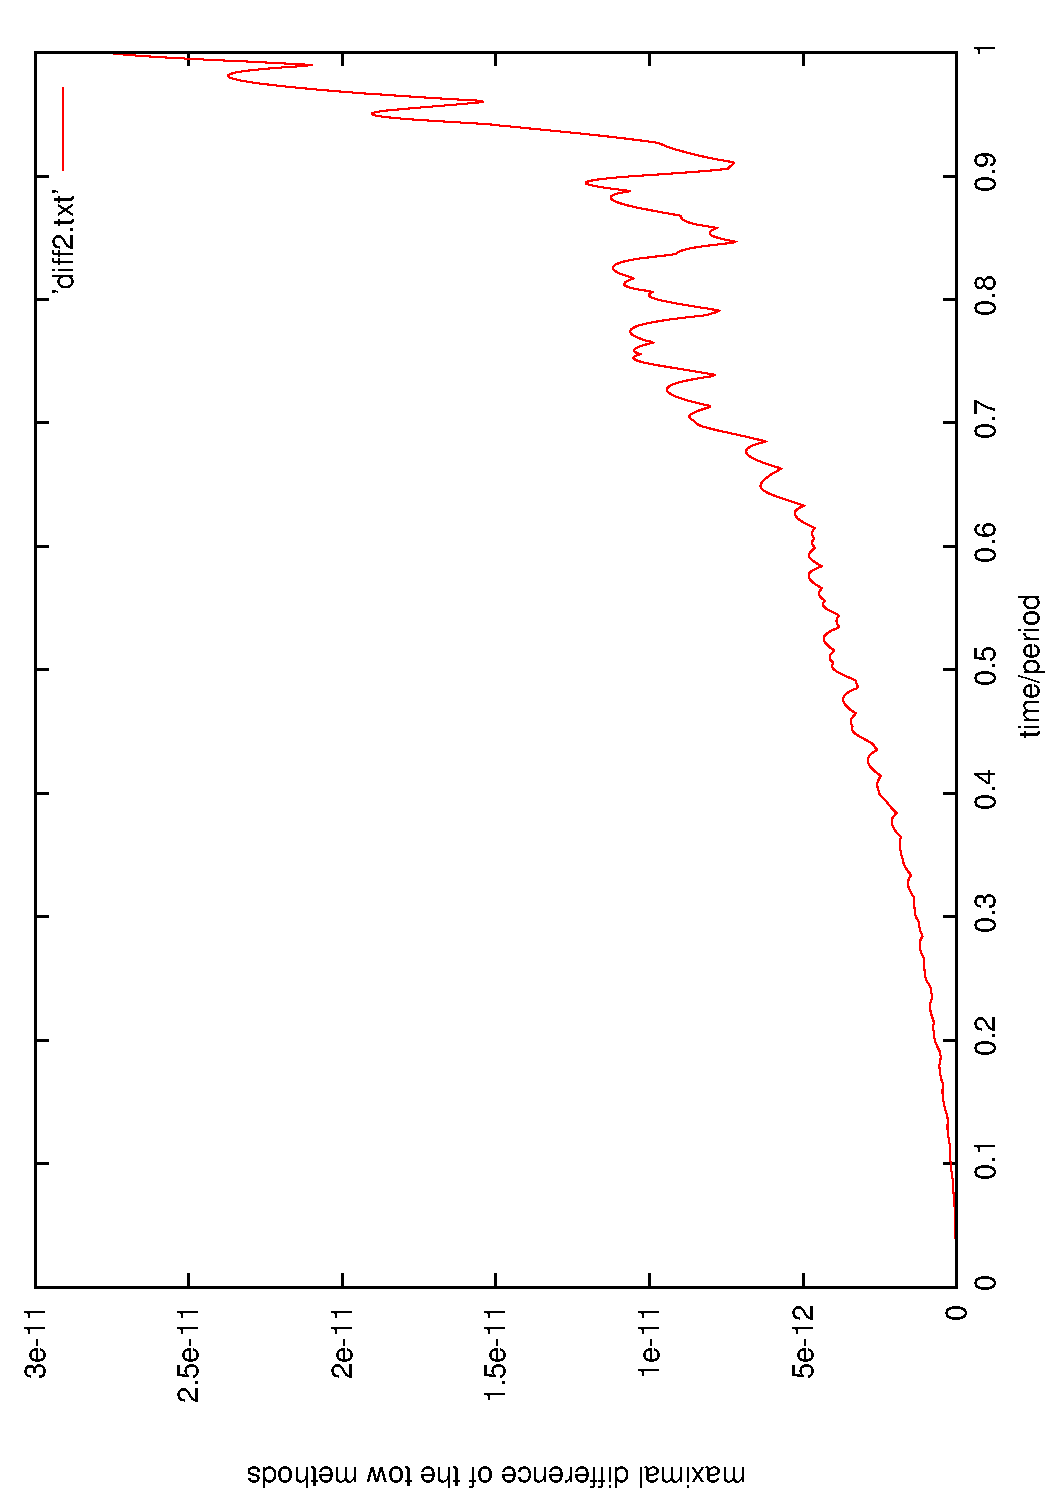
\includegraphics[angle=-90,width=0.5\textwidth]{diff-eps-converted-to.pdf}
 \caption{the maximal difference of the fourier modes for one period along the periodic orbit
  $T10.25$.}
 \label{fig:xiong_sdmfft_dif}
\end{figure}

\clearpage

%%%----------------------------------------------------------------------------
\subsubsection{Chebyshev Differential Matrix [Xiong Ding 2013-09-25]}
We know that the Discrete Fourier transform is a good tool to interpolate a periodic function,
 but what if the function is not periodic? Suppose there is a function $f(x)$ defined in $[-1,1]$.
 We make $f(x)$ to be periodic in
 $(-\infty, \infty)$ with period $2$ just by extending its value in $[-1,1]$ in two directions, and
 then use Fourier Differential Matrix to calculate its derivative in $[-1,1]$. However,
 this is a bad idea
 because extended function is not smooth now at points $x=\dots, -3,-1,1,3,\dots,$, which will result
 in the lose of accuracy of Fourier Differential Matrix.

 Another choice is to use polynomials $p(x)=a_{0}+a_{1}x+\dots+a_{N}x^{N}$ to interpolate $f(x)$
 in $[-1,1]$. Suppose there are $N+1$ sample points $x_{j},\quad j=0,1,2 \dots ,N$, then
 the error associated with polynomial interpolation is:
 \[
  err(x)=f(x)-p(x)=\frac{f^{N+1}(\varepsilon)}{(N+1)!}\Pi_{i=0}^{N}(x-x_{i})
 \]
 So a good interpolant will try to minimize $\Pi_{i=0}^{N}(x-x_{i})$.
 Now we turn to the question of how to choose sample points.

 \begin{enumerate}
  \item Equispaced interpolant: $x_{i}=\frac{2j}{N}-1,\quad j=0,1,\dots, N $. This is the choice
  emergeing in my mind the first time I think of interpolant, but it is not a good candidate for
  sample points, because the oscillations near the boundery will get worse
  when $N$ increases, which is called Runge phenomenon. At the same time, this method is less accurate
  than Chebyshev interpolant.
  For example, choosing $x=(N-1)/N$ and $N=30$ we have
  \[
   |\Pi_{i=0}^{N}(x-x_{i})|= \frac{(2N-1)!!}{N^{N+1}}\approx 4.7\times 10^{-6}
  \]


  \item Chebyshev interpolant: $x_{j}=\cos(\frac{j\pi}{N}), \quad j=0,1,2,\dots N$.
  These points are the maximal or minimal points of $N_{th}$ order Chebyshev polynomial:
  $T_{N}(x)=\cos(N\cos^{-1}(x))$, so they are (except $x_0$ and $x_N$)
  the zeros of $\frac{dT_{N}(x)}{dx}=NU_{N-1}=N\sin N\theta/\sin\theta$, where $U_{N-1}$
  is the second type Chebyshev polynomial and $x=\cos\theta$.
  \begin{align*}
   \prod_{i=0}^{N}(x-x_{i}) &=(x-x_0)(x-x_N)\prod_{i=1}^{N-1}(x-x_{i})\\
   &=\frac{1}{2^{N-1}}\frac{\sin N\theta}{\sin\theta}(x-1)(x+1)\\
   &=\frac{-1}{2^{N-1}}\sin N\theta \sin\theta
  \end{align*}

  The coefficient $1/2^{N-1}$ comes from the following fact: the highest order
  in $T_{N}(x)$ is $2^{N-1}x^{N}$ because of the recursive relation
  $T_{N}(x)=2xT_{N-1}(x)-T_{N-2}(x)$ and initial conditions $T_{0}=0,\quad T_{1}=x$;
  meanwhile, from $\frac{dT_{N}(x)}{dx}=N\sin N\theta/\sin\theta$ we know the highest order
  coefficient in  $\sin N\theta/\sin\theta$ is also $2^{N-1}$. Therefore, coefficient
  $1/2^{N-1}$ is required to rewirte $\prod_{i=0}^{N}(x-x_{i})$.

  \[
   |\prod_{i=0}^{N}(x-x_{i})|=\frac{1}{2^{N}} |sin N\theta \sin\theta| \leq \frac{1}{2^{N}}
  \]

  When $N=30$,  $\frac{1}{2^{N-1}}\approx 1.8\times 10^{-9}$. Now we can see that Chebyshev interpolant
  is superior to equispaced interpolant. If larger $N$ is choosen, the accuracy of Chebyshev interpolant
  is far better than that of equispaced interpolant. More importantly,
  Chebyshev interpolant circumvents the
  Runge phenomenon.


\end{enumerate}

  We now need to write down the specific form of polynomial that interpolate the discrete set
  $u_{j}=u(x_j),j=0,1,\dots,N$ at points $x_{j}=\cos(\frac{j\pi}{N})$, which is trivial:
  \begin{equation}
   P(x)=\sum_{j=0}^{N}p_{j}(x)u_{j}=\sum_{j=0}^{N}u_{j}\frac{\prod_{k\neq j}(x-x_{k})}{\prod_{k\neq j}(x_{j}-x_{k})}
  \end{equation}

  Obviously, $p_{j}(x_{i})=\delta_{i,j}$. Define $a_{j}=\prod_{k\neq j}(x_{j}-x_{k})$; thus we have:
  \[
   \frac{p_{i}(x)}{x-x_{j}}=\frac{a_j}{a_i} \frac{p_{j}(x)}{x-x_{i}}
  \]

  In order to calculate $dP(x)/dx$, we can use
  identity $\frac{d(\ln p_{j}(x))}{dx}=\sum_{k\neq j}(x-x_{k})^{-1}$. Therefore,
  \begin{align*}
   \frac{dP(x)}{dx} &= \sum_{j=0}^{N}p_{j}(x)\sum_{k\neq j}\frac{1}{x-x_{k}}u_{j}\\
   &=  \sum_{j=0,j\neq i}^{N}p_{j}(x)\sum_{k\neq j}\frac{1}{x-x_{k}}u_{j}+
   p_{i}(x)\sum_{k\neq i}\frac{1}{x-x_{k}}u_{i}\\
   &=  \sum_{j=0,j\neq i}^{N}[p_{j}(x)\sum_{k\neq j,k\neq i}\frac{1}{x-x_{k}}u_{j}+
   p_{j}(x)\frac{1}{x-x_{i}}u_{j}]+p_{i}(x)\sum_{k\neq i}\frac{1}{x-x_{k}}u_{i}\\
  \end{align*}

  Evaluated at point $x_{i}$, it becomes
  \begin{align*}
   & \frac{dP(x_{i})}{dx}\\
   & =\sum_{j=0,j\neq i}^{N} p_{j}(x_{i})\frac{1}{x-x_{i}}u_{j}
   +p_{i}(x_{i})\sum_{k\neq i}\frac{1}{x_{i}-x_{k}}u_{i}\\
   & =\sum_{j=0,j\neq i}^{N}\frac{a_i}{a_j}\frac{p_{i}(x_{i})}{x_{i}-x_{k}}u_{j}
   +p_{i}(x_{i})\sum_{k\neq i}\frac{1}{x_{i}-x_{k}}u_{i}\\
   & =\sum_{j=0,j\neq i}^{N}\frac{a_i}{a_j}\frac{1}{x_{i}-x_{k}}u_{j}
   +\sum_{k\neq i}\frac{1}{x_{i}-x_{k}}u_{i}\\
  \end{align*}

  Therefore, we can write down the Chebyshev Differential matrix:
  \[
   D_{i,j}=
   \begin{cases}
    \frac{a_{i}}{a_{j}(x_{i}-x_{j})} & (i\neq j)\\
    \sum_{k\neq i}\frac{1}{x_{i}-x_{k}} & (i=j)
   \end{cases}
  \]

  The next step is to determine $a_{i}/a_{j}$ and $\sum_{k\neq i}\frac{1}{x_{i}-x_{k}}$. Define
  $$A(x)=\prod_{i=0}^{N}(x-x_{i})$$. From previous discussion, we know
  \[
   A(x)=\frac{-1}{2^{N-1}}\sin N\theta\sin\theta
  \]
  where $\theta=cos^{-1}(x)$.

  \textbf{Claim 1}: $$A^{'}(x_{j})=a_{j}=\prod_{k\neq j}(x_{j}-x_{k})$$
  proof: $$A^{'}(x)=\sum_{j=0}^{N}\prod_{k\neq j}(x-x_{k})\Rightarrow
  A^{'}(x_{j})=\prod_{k\neq j}(x_{j}-x_{k}) $$

 \textbf{Claim 2}: $$\frac{A^{''}(x_{j})}{2A^{'}(x_{j})}=\sum_{k\neq i}\frac{1}{x_{i}-x_{k}}$$
 proof:
 \begin{align*}
 & A^{''}(x)=\sum_{i=0}^{N}\sum_{j\neq i}\prod_{k\neq i, k\neq j}2(x-x_{k})\\
 \Rightarrow & A^{''}(x_{j})=2\sum_{i\neq j}\prod_{k\neq i, k\neq j}(x_{j}-x_{k})\\
 \Rightarrow & \frac{A^{''}(x_{j})}{2A^{'}(x_{j})}=
 \frac{2\sum_{i\neq j}\prod_{k\neq i, k\neq j}(x_{j}-x_{k})}{2\prod_{k\neq j}(x_{j}-x_{k})}
 =\sum_{k\neq i}\frac{1}{x_{i}-x_{k}}
  \end{align*}

 The next step is easy: just evaluate $A^{'}(x_j)$ and $A^{''}(x_j)$. You can turn to chain rule
 to make life easier: $dA(x)/dx=dA(\theta)/d\theta \cdot d\theta/dx$. Meanwhile,
 $A^{'}(x)$ and $A^{''}(x)$ are singular at points $x=\pm 1$, so you can just take the limit
 $\lim_{x\to \pm 1}$ to get the values.

 In summary,
  \[
   -2^{N-1}A^{'}(x_j)=
   \begin{cases}
    2N & (j=0)\\
    2(-1)^{N}N & (j=N)\\
    (-1)^{j}N & (j\neq 0,N)
   \end{cases}
  \]

  \[
   -2^{N-1}A^{''}(x_j)=
   \begin{cases}
    \frac{4N^3+2N}{3} & (j=0)\\
    (-1)^{N}\frac{4N^3+2N}{3}  & (j=N)\\
    \frac{(-1)^{N+1}Nx_{j}}{1-x_{j}^{2}} & (j\neq 0,N)
   \end{cases}
  \]

  Eventually, we can write down the explicit formula for Chebyshev Differential matrix:
  \[
   D_{ij}=\frac{c_i}{c_j}\frac{(-1)^(i+j)}{x_{i}-x_{j}} \quad i\neq j
  \]
  \[
   D_{jj}=\frac{-x_{j}}{2(1-x^{2}_{j})} \quad j\neq 0,N
  \]
  \[
   D_{00}= \frac{2N^2+1}{6} ,\quad D_{NN}= -\frac{2N^2+1}{6}
  \]




%%%%%%%%%%    end of the differential matrix part     %%%%%%%%%%%%%%%%%%%%%%%%%%%%




\section{Daily log}
\label{sect:dailyBlXD}

This section is the daily (or at least, bi-weekly)  log of the Xiong Ding's
work.

\begin{description}

\item[2013-06-27 Predrag] Xiong Ding  <dingxiong203@gmail.com>,
1. year Georgia Tech physics graduate student, joined the
collaboration as a summer research project.
Xiong Ding will enter notes on his day-to-day progress into this log.

\item[2013-06-27 Evangelos] Maybe Xiong Ding could start with Francesco
    \etal\ review paper\rf{GiChLiPo12} instead of the blog? Francesco
    gave a talk here and made it seem very easy task to implement the
    method for a system of ODEs and also his paper seems readable.
    \\
{\bf [2013-06-27 Predrag]}
I agree, that's why the paper is referred to in the 1. line of
\refsect{sect:introXD} :) So does Kazumasa, see the next entry.

\item[2013-06-27 Kazumasa  to Xiong Ding]
Great! Please read (apart from ChaosBook.org)
%Francesco
Ginelli \etal\rf{ginelli-2007-99}
\HREF{http://prl.aps.org/abstract/PRL/v99/i13/e130601}{PRL}, and the
\HREF{http://arxiv.org/abs/1212.3961}{long follow-up paper}\rf{GiChLiPo12},
(much more detailed than the PRL).
Otherwise you will not understand anything on the codes (and the project).

\item[2013-06-27 Predrag]
I agree with Kazumasa: you want to write your own code,
but not necessarily reinvent the wheel. There is KS code various
places in this svn repository, for example in
\texttt{siminos/matlab/}, that you might want to compare performance
of your code with. Evangelos can help you with that.


\item[2013-06-14 Predrag]
Take a few days to read through this blog, and then we talk,
Skype or in person.
Enjoy :)

To start working on the covariant vectors project,
the
\HREF{http://www.cns.gatech.edu/CNS-only/subv.html} {subversion repository}
(type   cnsuser   cnsweb) is called
\begin{verbatim}
svn checkout svn://zero.physics.gatech.edu/siminos
username, password:     xiong and Lyapunov
\end{verbatim}
Chris Marcotte <christopher.marcotte@gmail.com, can help you get
started. Daniel Borrero dborrero@gatech.edu and Qi Ge
    qge30@gatech.edu also know how to do it. Failing that, I'll help
you via Skype predragcvitanovic.

\item[2013-07-03 Xiong Ding] Here is my first blog post:
A question about the \KS\ equation.
It seems that there are many versions of KS equation,
and some of them are totally different.
The one you used in \refref{SCD07}, ``On the state space geometry of
the KS flow in a periodic domain'' is
\beq
 u_t=-\frac{1}{2}(u^2)_x-u_{xx}-u_{xxxx}
\ee{XD-KSeSCD07}
However, the
equation in \refref{KNSks90}, ``Back in the saddle again: a computer
assisted study of the KS equation'' is:
\beq
 u_t+4\bigtriangleup^2 u
    +\alpha (\bigtriangleup u +\frac{1}{2}(\bigtriangledown u)^2)=0
\ee{XD-KSeSCD07}
The first order term is different.

\item[2013-07-04 Predrag] That is always annoying when one reads
KS literature - I asked that Evangelos include various transformations
in his thesis, but I cannot find that text, only this:
``The parameter $\alpha$ of \refrefs{KNSks90,ksgreene88} is
related to the system size by $\tildeL=\sqrt{\alpha/4}$.''

In Evangelos
\HREF{../blog/blog.pdf} {blog} we write

``
The {1\dmn} \KSe\ as given in \refrefs{ku,siv} is (up to overall scaling
factors):
\beq
    y_t=-y_x^2/2-y_{xxxx}-y_{xx}
\,,\qquad       x \in [0,L]
\,,
    \label{eq:KSeOR}
\eeq
with periodic boundary conditions in the $[0,L]$ interval. The form used
here
\beq
    u_t=uu_x-u_{xxxx}-u_{xx}
\,.
    \label{eq:KSeAP}
\eeq
is obtained from \refeq{eq:KSeOR} by differentiating with respect to $x$
and setting \PCedit{$u=-y_x$}.
In study of {1\dmn} \KS\ \eqva\ $x$ in \refrefs{LanThesis,ksgreene88}
is interpreted as ``time", so $y$ is a height of a front,
and $y_x$ its ``velocity".
In the literature  both forms of the equation are
referred to as the \KSe.
''

In Evangelos blog I rescued the text that he did not use in his thesis,
copied below.
Let us know whether this resolves your quandary,
and please do remember to include this in your project
report, so it is available to future students (I should really
include it into an appendix to ChaosBook...)            \toCB

\item[2007-01-20 Evangelos]
Notes on Greene and Kim\rf{ksgreene88}. A copy is in ChaosBook.org/library,
\HREF{http://chaosbook.org/library/index.html}{click here}.

\noindent\textbf{\Eqva\ according to Greene and Kim:}
%
The form of \KSe\ studied by Greene and Kim\rf{ksgreene88} is
\beq
    y_t=-4y_{xxxx}-\alpha\left(y_{xx}+\frac{1}{2}y_x^2
            -\frac{1}{4\pi}\int_0^{2\pi}y_x^2\ dx\right)
\,,\qquad       x \in [0,2\pi]
\,,
    \label{eq:KSeGreeneKim}
\eeq
with  periodic boundary condition on the interval $[0,2\pi]$.
Mean elastic energy density of a spatial profile $y(x,t)$ is defined by
\beq
    E=\frac{1}{2\pi}\int_0^{2\pi}y_x^2\, dx\,.
    \label{KSenergy}
\eeq
% \ES{This definition does not only apply to equilibria. Greene and
% Kim also study the transfer of energy between modes
% in non-stationary trajectories.}.
Taking the derivative of \refeq{eq:KSeGreeneKim}
with respect to $x$ and substituting $y_x=-u$ leads to
\[
    u_t=4u_{xxxx}+\alpha\left(u_{xx}-uu_x\right)
\,.
\]
Rescaling
\beq
    \tilde{x}=\frac{\sqrt{\alpha}}{2} x
\,,\qquad
    \tilde{t}=\frac{\alpha^2}{4} t
\,,\qquad
    \tilde{u}=\frac{2}{\sqrt{\alpha}} u
    \label{eq:GKscale}
\eeq
brings the Greene-Kim equation to the form \refeq{eq:KSeAP} used here.
The dimensionless system size $\tildeL=L/2\pi$ is related to
the Greene-Kim parameter
through $\tildeL=\sqrt{\alpha}/2$.
The system size $L=22$ studied here corresponds to $\alpha=49.0395$.

The ``kinetic energy'' reads in our units:
\PC{shouldn't there be a prefactor $\frac{1}{2}$?}
\beq
    \tilde{E}=\frac{1}{L}\int_0^{L}\tilde{u}^2\, d\tilde{x}\,.
\eeq
Integrating \refeq{ks} in $[0,L]$ we get $c=\tilde{E}$,
since the terms involving $u_x$ and $u_{xxx}$ vanish due to periodicity.
From the scalings \refeq{eq:GKscale} we have $\tilde{E}=\frac{4}{\alpha}E$.


\item[2013-07-03 Xiong Ding] In \refref{SCD07} you point out KS
    equation is Galilean invariant: if $u(x,t)$ is a solution, then
    $u(x-ct)-c$ is also a solution. but I am confused, because when I
    substitute it into the equation I get a minus sign. If I change the
    form to be $u(x-ct)+c$, then it is OK.

\item[2013-07-04 Predrag] Thanks for noticing this - you are correct, see
2nd paragraph of Section ChaosBook {\em 26.1.1 Scaling and symmetries.}
(all ChaosBook section and eq.~numbers refer to the stable
\HREF{http://chaosbook.org/version14/pdf.shtml} {version 14} of Dec.
31 2012). The error has propagated from Evangelos
\HREF{http://chaosbook.org/projects/theses.html} {thesis},
{\em section 5.1.2 Symmetries of Kuramoto-Sivashinsky system} to the article.

Embarrassing, but too small an error to change the arXiv version of \refref{SCD07}
(though Evangelos could fix it in his thesis)...

Now I note that the ChaosBook {\em Exercise
26.1.
Galilean invariance of the Kuramoto-Sivashinsky equation} is also in error.
As you are checking the KS papers anyhow, you would help me a lot if you also
checked {\em Chapter 27 Turbulence?} as you went along - that chapter is still
only a draft, has been very hard to write up concisely...
Please correct \refexer{exer:GalInv}, write up the solution
(I'll transfer it back to ChaosBook).                   \toCB
\\{\bf [2013-07-12 Xiong Ding] done.}

\item[2013-07-04 Predrag] I assume we are going to work on the
    covariant vectors project, so please try to learn how to check out
    the repository (see {\bf [2013-06-14 Predrag]} above).

\item[2013-07-05 Xiong Ding] I tried to read the \emph{Appendix C - Linear
    Stability} in ChaosBook, but it was hard for me to understand the
    `Fundamental matrix' and the `Dual space'. I don't know what book
    or paper covers this material. Could you give me some suggestion?

For now we do use either for time being - `fundamental matrix' is
discussed a bit in
    \PC{the pdf file text in purple is a hyperlink - click on it to
    see the file I am referring to...}
\emph{\HREF{http://chaosbook.org/paper.shtml\#stability} {Section 4.3} A
linear diversion}, but only for completeness, and `dual spaces' we might
have to define once we start using norms other than $L2$ for \KS. For
now, ignore them. We should remember to rewrite `fundamental matrix'
discussion in
\emph{\HREF{http://chaosbook.org/paper.shtml\#appendStability} {Appendix
C} - Linear Stability} later on - I agree that it is confusing.

\item[2013-07-05 Xiong Ding]
You want me to check the material in Chapter 27. I
will try, but now I only finish reading the first eight chapters. I am
\PCedit{stuck}
    \PC{here purple indicates Predrag's edit. Nobody's perfect.}
at Chapter 9 (groups and symmetries). So I am not sure when I can
understand Chapter 27.

\item[2013-07-05 Predrag] Chapter 27? Do you mean \emph{
\HREF{http://chaosbook.org/paper.shtml\#PDEs}{Chapter 26} - Turbulence?}
ChaosBook is not sequential - to understand this chapter you only need
chapters 2-6 and 11-12. For the time being you can skip
{\em Chapter 9 - World in a mirror} and
{\em Chapter 10 - Relativity for cyclists}, jump straight from
{\em Chapter 6 - Lyapunov exponents} to {\em {Chapter 26} - Turbulence}.

\item[2013-07-07 Predrag] Our man Xiong
(\HREF{http://www.youtube.com/watch?v=0t1_usmB30s}{agent 007})
has mastered VPN and can check out / commit this repository.

\item[2013-07-10 Xiong Ding]
% I am not sure whether my system can handle VPN now.
The structure of this repository is very complicated.

\item[2013-07-07 Predrag to 007] For now you care only about
\begin{verbatim}
siminos/lyapunov/blog.tex
\end{verbatim}
 but the wisdom accrued
elsewhere in \texttt{siminos} repository might come in handy -
we'll point you to relevant files as the need arises. The
published papers are in the blog - you might find that useful
for clip \& paste, rather than typing everything from the scratch...

\item[2013-07-11 Xiong Ding] Yesterday I talked with Prof. Predrag and I was
sceptical about the $1/2$ coefficient in the Fourier transform
\refeq{expan} of the \KS\
equation \refeq{XD-KSeSCD07}.
\[
 u_t=-\frac{1}{2}(u^2)_x-u_{xx}-u_{xxxx}
 \,.
\]
We perform Fourier transform:
\[
 u(x,t)=\sum_{k=-\infty}^{+\infty} a_{k}(t)e^{ikx/\tilde{L}}
\]
For the nonlinear term $-\frac{1}{2}(u^2)_x$, we get
$-i\frac{q_k}{2}\sum_{m=-\infty}^{+\infty} a_{m}a_{k-m}$,
where $q_k=k/\tilde{L}$. It has the form of
convolution, which comes from one property of Fourier transform.
Now I try to write it down in detail:
\begin{align*}
 -\frac{1}{2}(u^2)_x &=-uu_x \\
 &=-\sum_{m=-\infty}^{+\infty} a_{m}(t)e^{imx/\tilde{L}}
 \sum_{n=-\infty}^{+\infty} \frac{in}{\tilde{L}} a_{n}(t)e^{inx/\tilde{L}}\\
 &=-\sum_{m=-\infty}^{+\infty}\sum_{n=-\infty}^{+\infty} iq_{n} a_{m}(t)e^{iq_{m}x}a_{n}(t)e^{iq_{n}x}\\
 &=-\frac{i}{2}\sum_{m=-\infty}^{+\infty}\sum_{n=-\infty}^{+\infty}
 (q_{n}+q_m) a_{m}(t)e^{iq_{m}x}a_{n}(t)e^{iq_{n}x}\\
 &=-\frac{i}{2}\sum_{m=-\infty}^{+\infty}\sum_{n=-\infty}^{+\infty} q_{n+m} a_{m}(t)a_{n}(t)e^{i(q_{n}+q_m)x}
\end{align*}
If we take out the coefficient of term $e^{iq_{k}x}$, it will give
$-i\frac{q_k}{2}\sum_{m=-\infty}^{+\infty} a_{m}a_{k-m}$, thus the
Fourier transform \refeq{expan} is correct.

\item[2013-07-12 Xiong Ding] Wrote up solution to \refexer{exer:GalInv},
{\em Galilean invariance of the \KSe.}

\item[2013-07-12 Predrag] Created the research level \refexer{exer:locGalInv},
{\em Local Galilean invariance of \KS.}

\item[2013-07-12 Predrag to Xiong Ding]
I have \HREF{http://www.bmp.ds.mpg.de/philip-bittihn.html} {Philip
Bittihn} PhD thesis\rf{BittihnThesis} for you. Philip has been
co-advised by Flavio, and in his thesis he carries out covariant
Lyapunov vector calculations based on Ginelli
\etal\rf{ginelli-2007-99} method. He applies them to the Barkley
model (I have asked Kamal Sharma to do that), and to the Fenton-Karma
model (Chris Marcotte is working on that). I suggest you study that
part of the thesis, and after you have read relevant sections, we can
ask Philip to give us informal webinar, where he can answer your
questions.

\item[2013-07-22 Predrag to Xiong Ding] Are you OK, or should I ask police to check
your apartment :) Have not seen anything in the blog since 2013-07-12. Let's
make a schedule for updates: how about no later than 5PM on Tuesdays and Thursdays?
Propose some other times if these are not optimal...

I'm in Chicago and
\HREF{http://www.cns.gatech.edu/~predrag/schedule/travel.txt} {Woods Hole}
until Aug 17, but we can meet on Skype whenever you would like to discuss
something. I have asked building manager to give you temporarily a key to
W501B (desk to the left, as you enter, is empty), until Aug 7.
Thereafter Greg Byrne, our new
postdoc arrives. If this is too much trouble for too short time, do not move.
I am away, but Chris and Adam are nearby, and they are good to talk to.

\item[2013-07-22 Xiong Ding to Predrag] I am writing the code these
    days. I follow the instructions in paper \refref{ks05com} to update
    the \KS\ equation in \statesp\ and the movement in tangent space. I
    record the diagonal elements of the up-triangular matrix to
    calculate the Lyapunov exponents. The code written in Matlab gave
    me inconsistent results; while the code written in C++ doesn't work
    because of overflow. I am sorry I didn't update the blog these days
    because I haven't achieved anything sensible.

\item[2013-07-22 Predrag] This is too telegraphic. People just say 'Lyapunov
exponents' without a definition, usually meaning something that is not
a 'Lyapunov exponent'. Are you computing
stability multipliers (or stability exponents, logarithms of multipliers
divided by
time) of \jacobianMs, or are computing the long time limits of
singular values of (\jacobianM$\transp{)}\times($\jacobianM)?
If you do not understand the question (and that is OK - the literature is
very confusing), reread stability and Lyapunov
chapters of ChaosBook.

\item[2013-07-22 Xiong Ding to Predrag] Sorry for my telegraphic report. I mean I update
the orthogonal tangent vectors for several steps and then conduct $QR$ factoring.
I record the diagonal elements of the up-triangular matrix $R$ and use the formula
in \rf{GiChLiPo12} to calculate these exponents. So it refers to the stability multipliers
of \jacobianMs.
\[
 \lambda_i=\lim_{T\to \infty} \frac{1}{T} \sum_{h=0}^{T-1}
  \ln\gamma_{k,n+hk}^{(i)}
 \,.
\]
I uploaded my C++ code to folder \texttt{xiong/c/}
and two Matlab codes to folder \texttt{\texttt{xiong/matlab/}}.
One of them, \texttt{etdrk4.m}, is just a copy from \refref{ks05com}. I tried to increase
the total time and found that the recorded data overflew. I changed the length of space period
to be 22 in other two files, but the exponents were different from those in paper \refref{SCD07}.


\begin{quote}
``[...] Indeed, numerically the covariant Lyapunov
vectors\rf{ginelli-2007-99} of the $L=22$ chaotic attractor separate
into 8 ``physical'' vectors with small Lyapunov exponents
$(\Lyap_j) = (0.048,$ 0, 0, $-0.003$, $-0.189$, $-0.256$,
$-0.290$, $-0.310$),
and the remaining 54 ``hyperbolically isolated'' vectors with rapidly
decreasing exponents
$(\Lyap_j)
= (-1.963$,   $-1.967$,   $-5.605$,   $-5.605$,  $-11.923$,  $-11.923$,
 $\cdots) \approx -(j/\tildeL)^4$,
in full agreement with the Yang \etal\rf{YaTaGiChRa08} investigations
of KS for large systems sizes.
 [...]''
\end{quote}

Maybe the problem lies in the my code structure, or I misunderstand the algorithm described in
\rf{GiChLiPo12}. Also, I am wondering whether it is correct to select an arbitrary inital
condition for the dynamics in phase space because it may not enter the ``inertial manifold''.

I think I should study paper \refref{SCD07} thoroughly first and then turn to coding again. I
cannot stand writing another hundreds of lines in C++ for next few days.:)

\item[2013-07-22 Xiong Ding]
Now I try to focus on those codes and locate the problems with them.
Do you have any suggestion?

\item[2013-07-22 Predrag] It's a big project, and these codes are not written
in a week. One step at the time. Before implementing them for \KS,
test them on simple things, like Lorenz and R\"ossler. Write down here,
in the blog, the
formulas your code is supposed to implement. Save programs
(but usually not data other than parameters, initial conditions and such,
especially if it takes lots of space)
and document them in your
directories under \texttt{siminos/xiong/} so Kazumasa and/or Evangelos
can test them, help you debug them. Once the problem is explained
here, ask Kazumasa for advice (I have not done serious coding in years :).

\item[2013-07-22 Predrag] For a few suggestions for simple models to
test on, see \refsect{sect:CovVecs}.

\item[2013-07-23 Kazumasa via Predrag]
I cannot read and update the blog while travelling, but has Xiong has
tried my code? My C++  code \texttt{lyap-upo.cpp} and \texttt{README.txt}
are in \texttt{siminos/kazz/code/}. You compile and run it as C++. Note
that, though I extracted a part of my long code relevant to our project,
it contains many functions which you probably will not need.

I strongly recommend that you write your own code from zero, without
reference to mine. This is the best way to learn what's going on in
the code. Don't try to write a code with full functionality from the
beginning, but start with a minimal code, which only computes, say,
Lyapunov exponents.
Confirming that this works as you expect, you can add a code to compute
the covariant vectors from a simple forward-backward process (and
check if the exponents values computed from the covariant vectors
agree with those from the Gram-Schmidt method). For practical use,
you have to implement the "block-by-block" computation of the
vectors, to overcome memory issues (see discussions in Sec. 4.2 in
Ginelli \etal\rf{GiChLiPo12}, \arXiv{1212.3961}). This is
the first step you should reach in this project.

For numerical integration of the KS equation, I used the
operator-splitting algorithm (Adams-Moulton method + Heun's method),
typically with time step 0.005. For more detail, read Sect.~II~A in
Takeuchi \etal\rf{TaGiCh11}. Stiffness matters, implicit methods are
common ways to overcome this problem,
 and that's why I used the Adams-Moulton method. To further improve,
it's better to split the linear and non-linear terms
 by the operator splitting method and use the implicit method only to
 the linear terms where the stiffness is.
I'm not saying that my algorithm is the best way to simulate the KS
equation, but at least it's suited to practical use.

\item[2013-06-27 Predrag  to Xiong Ding]
A discussion of stiffness in integrating PDEs can be found
\HREF{http://www.pvv.ntnu.no/~berland/talks/berland05expintro.pdf}
{here}. \HREF{http://www.math.ntnu.no/num/expint/} {Here} is Matlab
package for testing 47 (!) schemes.

Study the methods described in
\HREF{http://www.cns.gatech.edu/~predrag/papers/SCD07.pdf}
{Appendix A} of \refref{SCD07}.
%The authors have lots of experience and they went to the
%    trouble of explaining the best methods they know, so why not read
%    them and implement them?

The plot of what you get for $L=22$
Lyapunov spectrum should confirm the published results (see
{\bf [2009-09-13 Ruslan]} on \refpage{sect:LyapKS},
\reffig{fig:lyapSpecCLG}, \reffig{fig:lyapSpec1},
\reffig{fig:lyapSpec}, and \reftab{tab:ks22shad}) and the
figure\PC{which one? Always state the number} in Kazumasa \etal\
paper\rf{TaGiCh11} (read it
\HREF{http://chaosbook.org/library/KoSa11.pdf} {here}).

\item[2013-06-27 Ruslan]
You can use the method developed by Cox and
Matthews\rf{cox02jcomp} and improved by Kassam and
Trefethen\rf{ks05com}, where the linear part is integrated exactly.
My Matlab code {\tt ksfmetd2.m} is based on this method and it is
stable and reasonably accurate with time step as large as 0.25.  It
also solves variational problem, so can be used to calculate Lyapunov
exponents.  See {\tt ksfmlyap.m} in {\tt siminos/matlab/ruslan/},
read {\tt 00ReadMe.txt}.  If you want to compute Lyapunov exponents
using the standard GS procedure, the relevant code is in {\tt
ksdupo.m} in the same folder (look for the cell "\%\% Compute
Lyapunov exponents of KS (using ksfmlyap and GS)").

\item[2013-06-27 Predrag]
Ruslan uses the same \KSe\ convention as Kassam and
Trefethen\refrefs{ks05com}. I have saved the Trefethen Matlab code
\HREF{http://chaosbook.org/extras/Trefethen/kursiv.m} {here}. Perhaps
you want to c++ it, see how it runs for you, or run it in Matlab and
compare with your code. There might be something else useful on
\HREF{http://chaosbook.org/extras/}{ChaosBook.org/extras} homepage,
for example the simulations by the spring 2007 GaTech chaos class.
You can search the blog for 'Trefethen' for other discussions
(Kazumasa has reservations about the Trefethen\rf{ks05com} algorithm,
but Ruslan is OK with it).
Siminos has other codes, if needed, on a different repository.

\item[2013-01-21 Evangelos] The \KS\ data you need is in \\
\texttt{siminos/matlab/ruslan/kse22orbits.mat},
\\
in a structure called \texttt{eq}.
Eigenvalues are in the field eq.eig and right
eigenvectors are in the field eq.evec. [e.g. eq(k).evec(:,1) is the
eigenvector which corresponds to the first eigenvalue eq(k).eig(1) of
the k'th equilibrium]. However, I have not used the data for a long
time so, it would be better if Ruslan verifies how the Fourier modes
are stored (I think that the numbers in a column vector correspond to
real and imaginary part of the Fourier modes
\[
 (a_1,\, b_1,\, a_2,\, b_2,\, \ldots a_N,\, b_N)
\]
and thus here there are $31+1$ complex Fourier modes (the zero'th mode
is not included)).

In order to get the left eigenvectors you will need to compute the
stability matrix.

If you run into problems or have questions please email me so that we
can arrange to talk through Skype.


\item[2013-06-27 Ruslan] To compute stability matrix in Matlab, use
\\
\texttt{siminos/matlab/ruslan/ksfm.m}:
\\ {\tt [f, df] = ksfm(0,eq(1).a,22.0)},
\\where {\tt df} will be the stability matrix of $EQ_1$.

The idea of the method is described in \refref{SCD07} Appendix A and
B.  The Jacobian matrix is calculated from (B.1) which uses solutions
of (A.4) and (A.6).  Matlab code {\tt ksfmetd2.m} solves (A.4) and
(A.6) simultaneously.  The Jacobian matrix is output in {\tt da}.
You don't need anything else.


\item[2013-07-23 Xiong Ding]
I don't understand one point of Appendix A in paper \rf{SCD07}.
After Fourier transform,
\[
 u(x,t)=\sum_{k=0}^{N} a_{k}(t)e^{ikx/\tilde{L}}
\]
we have relation $a_{N-k}^{~}=a_{k}^{*}$ and set $a_0=0$ due to Galilean
invariance, but why can we also set $a_{N/2}=0$ ?
\\
{\bf [2013-07-24 Predrag]} The first relation is due to the reality of
\( u(x,t) \). I suspect that the second one is due to the periodicity
\( u(x,t) = u(x+L,t) \). Let me know if I am wrong?

\item[2013-07-24  Xiong Ding]
Why both $a_{N/2}=0$ and $a_0=0$? I think $a_{N/2}=0$ comes from Galilean
invariance of \KS\ equation; while we set $a_0=0$ just for the
convenience to perform the discrete Fourier transform. It is not one
component of the Fourier spectrum because we are using discrete Fourier
transform to truncate the nonlinear term in continuous Fourier transform.
Am I right?

\item[2013-07-30 Evangelos to Xiong Ding]
$\dot{a}_0=0$ by Galilean invariance and thus $a_0$ is constant. We \emph{choose} this constant to be zero so that
the mean value of our solutions is zero. Otherwise you would get ``drifting solutions.''
$a_{N/2}=0$ is the DFT analog of $a_k=a^*_{-k}$, which holds in general for Fourier series of real data.
(This is discussed in my thesis.)

\item[2013-07-24  Xiong Ding] the initial condition of $T_{10.25}$ in
\\*
\texttt{siminos/matlab/ruslan/ks22f90h25t100.mat}
was used in my code. Hoping to get a
periodic graph, I failed. After scrutinizing my code carefully,
I could not find an error, so I suspected that maybe some variables
defined in Ruslan's code were differently
from mine.

I compared my code with \texttt{siminos/matlab/ruslan/ksfmetd2.m},
there is a major difference at the form of the coefficient before the nonlinear term.
Ruslan used \texttt{g = 0.5i*k*N}, but I prefer to \texttt{g=-0.5i*k}.
Such a difference results from the slightly different use of discrete Fourier transform
and the conjugacy of $a_k$, which is \PCedit{$a_{N-k}=a^{*}_k$}.

If we prefer the discrete Fourier transform defined in the Appendix A of
\refref{SCD07},
\[
 u(x,t)=F_N^{-1}[a]_n=\frac{1}{N}\sum_{k=0}^{N-1} a_{k}(t)e^{iq_{k}x_{n}}
\,,
\]
\KS\ equation will be transformed to
\[
 \dot{a_k}=(q_{k}^2-q_k^4)a_k-i\frac{q_k}{2}F_{n}[(F_N^{-1}[a])^2]_k
\,.
\]

Note that the nonlinear term is
\[
-i\frac{q_k}{2}F_{n}[(F_N^{-1}[a])^2]_k=-i\frac{q_k}{2}\frac{1}{N}\sum_{m=-\infty}^{+\infty}a_{m}a_{k-m}
\,.
\]
I think maybe Ruslan hopes the transformed equation is consistent with the form
\[
 \dot{a_k}=(q_{k}^2-q_k^4)a_k-i\frac{q_k}{2}\sum_{m=-\infty}^{+\infty}a_{m}a_{k-m}
\,,
\]
so he keeps the coefficient before the nonlinear term by $N$ times larger.

The sign of the coefficient is defined by whether you treat $\mathbf{a}(t_0)$ as inital condition or
$\mathbf{a}^{*}(t_0)$.


In conclusion, if I insist on my style, I should transform the initial condition $\mathbf{a}(t_0)$
for $T_{10.25}$  to $N\mathbf{a}*(t_0)$, but I think it is better to follow predecessors' style.

\item[2013-07-30 Evangelos to Xiong]
It seems everyone of us uses a different normalization of FFT and sometimes this leads to
confusion. I would suggest that you follow Ruslan's conventions so that you do not need to transform
his data. Also, if you write C++ or Fortran code, I recommend using the excellent FFTW library.

\item[2013-07-28  Xiong Ding] I tried to calculate the Floquet exponents of the \po\ $T_{10.25}$
according to the evolution law of \JacobianMs\ \refeq{XD-JacobianEq}.
I evolve the system for 10.25 time units, and get the \jacobianMs\ which is initially an identity matrix.
The Floquet exponents are defined as $\Lyap_i=\ln \ExpaEig_i /\period{}$, where $\ExpaEig_i$ is an
eigenvalue of $J^{10.25}$. What I got is:
\\

   0.23258 - 0.00000i          \\
   0.14955 + 0.12659i          \\
   0.14955 - 0.12659i          \\
   0.03606 - 0.09769i          \\
   0.03606 + 0.09769i          \\
   0.00000 + 0.00000i\\
   0.00000 + 0.00000i\\
  -0.12645 - 0.00000i          \\
  -0.26741 + 0.00000i          \\
  -0.31008 + 0.00000i          \\
  -2.08643 + 0.00031i          \\
  -2.08643 - 0.00031i          \\
  -3.75575 - 0.12337i          \\
  -3.85635 + 0.02976i          \\
         (the rest are commented out in the printout) \\
%  -3.89556 + 0.23714i\\
%  -3.96240 - 0.16580i\\
%  -3.98168 - 0.03617i\\
%  -4.25816 - 0.24501i\\
%  -4.32998 - 0.19698i\\
%  -4.35308 + 0.16783i\\
%  -4.37326 - 0.09470i\\
%  -4.51263 + 0.18201i\\
%  -4.59075 + 0.01169i\\
%  -4.65092 + 0.22378i\\
%  -4.72197 - 0.21302i\\
%  -4.75598 - 0.14938i\\
%  -4.77917 + 0.15105i\\
%  -4.91567 - 0.28930i\\
%  -4.99471 - 0.12117i\\
%  -4.96573 + 0.12500i\\
%  -5.07246 + 0.22152i\\
%  -5.17096 - 0.17295i\\

However, when I tried to check my result against the data in
\\
\texttt{siminos/matlab/ruslan/ks22f90h25t100.mat},
\\
I find they are different. The eigenvalues there are

      -0.59458 + 1.27298i\\
      -0.59458 - 1.27298i\\
      -1.00000 + 0.00000i\\
       1.00000 + 0.00000i\\
       0.10870 + 0.00000i\\
      -0.05706 + 0.03281i\\
      -0.05706 - 0.03281i\\
      -0.03366 + 0.00000i\\
       0.00000 + 0.00000i\\
       (the rest are all zeros) \\
   %   -0.00000 + 0.00000i\\
%       0.00000 + 0.00000i\\
%      -0.00000 + 0.00000i\\
%      -0.00000 + 0.00000i\\
%      -0.00000 + 0.00000i\\
%       0.00000 + 0.00000i\\
%      -0.00000 + 0.00000i\\
%      -0.00000 + 0.00000i\\
%      -0.00000 + 0.00000i\\
%       0.00000 + 0.00000i\\
%      -0.00000 + 0.00000i\\
%       0.00000 + 0.00000i\\
%       0.00000 + 0.00000i\\
%      -0.00000 + 0.00000i\\
%       0.00000 + 0.00000i\\
%      -0.00000 + 0.00000i\\
%      -0.00000 + 0.00000i\\
%      -0.00000 + 0.00000i\\
%      -0.00000 + 0.00000i\\
%      -0.00000 - 0.00000i\\
%       0.00000 + 0.00000i\\

I don't know the meaning of eigenvalues in this file. And, why are there
so many zeros?

\item[2013-07-30 Evangelos to Xiong]
The file under question provides Floquet multipliers (eigenvalues of the Jacobian). This is documented here in this blog, I think (but it's too hard to trace it).
The lack of a symmetric partner for your largest Floquet exponent indicates something might be wrong. When you integrate the trajectory, how close does it get to
the initial value? Also, please recheck your definition of Floquet exponents.

\item[2013-07-30 Predrag to Xiong] My guess is that you have not read
    Ruslan's instructions for how to read the data sets. As long as
    your integration of a periodic point on \po\ \PO{10.25} does not
    close after one period, there is no point of computing Floquet
    exponets; everything computed on a wrong orbit is wrong, right?
    Once your code verifies the periodicity (to machine precision, not
    to 1\%), then go for the Floquet exponents. What about plotting
    your Floquet exponents in the style of \reffig{fig:lyapSpec1} and
    other figures in the blog, and seeing how they compare with your
    exponents? How do you compare to \reftab{tab:ks22po10.25FloqExp}?
    If you search for 10.25 throughout this blog, you will find much
    discussion of this \po, and its properties.

\item[2013-07-30 Predrag to Xiong] The period of \po\
    \PO{10.25} is not $\period{}=10.25$ it is
    $\period{}=10.25336729174627$, or whatever full precision number
    you are given in Evangelos and/or Ruslan data sets. You are
    computing all properties of an invariant solution to machine
    precision, not to 1\% accuracy; the whole problem with the naive
    integration of \refeq{XD-JacobianEq} is that it can compute only a
    few leading Floquet multipliers / exponents, while the method you
    are going to adopt from Ginelli \etal\rf{GiChLiPo12} is supposed to
    give you {\em all} exponents to the full precision.

\item[2013-07-30 Predrag to Xiong] Please write out here explicitly, in
    formulas, Evangelos computation that gives $a_{N/2}=0$, so we are
    sure that you and Evangelos agree.

\item[2013-08-01 Xiong Ding to Predrag and Evangelos] Thank you for the analysis to my
problem and useful suggestions. I really appreciate your reply. :)

First, I want to write down my understanding on code \\
\texttt{siminos/matlab/ruslan/ksfmetd2.m} \\
and give my opinion about $a_{N/2}=0$.

\KS\ equation is
\[
 u_t=-\frac{1}{2}(u^2)_x-u_{xx}-u_{xxxx}
 \,.
\]
We perform a Fourier transform,
\begin{align*}
 \hat{u}_{k} &= F[u]_{k}= \frac{1}{L}\int_{0}^{L} u(x,t)e^{-iq_{k}x}dx\\
 u(x,t) &= F^{-1}[\hat{u}] = \sum_{k=-\infty}^{+\infty} \hat{u}_{k} e^{iq_{k}x}
\end{align*}
In the Fourier space the \KS\ equation is
\begin{align}
 \dot{\hat{u}}_{k} &= (q^{2}_{k}-q^{4}_{k})\hat{u}_{k}-\frac{iq_{k}}{2}F[(F^{-1}[\hat{u}])^{2}]_{k}\nonumber\\
 &= (q^{2}_{k}-q^{4}_{k})\hat{u}_{k}-\frac{iq_{k}}{2} \sum_{m=-\infty}^{+\infty} \hat{u}_{m}\hat{u}_{k-m}\nonumber\\
 & \doteq (q^{2}_{k}-q^{4}_{k})\hat{u}_{k}-\frac{iq_{k}}{2} \sum_{m=-N}^{N} \hat{u}_{m}\hat{u}_{k-m}\label{xfft1}
\,,
\end{align}
where in \refeq{xfft1}, I make a truncation of the wave number from $-N$ to $N$, which is just a approximation, and we have
a relation $\hat{u}_{-k}=\hat{u}_{k}^{*}$ since $u(x,t)$ is a real function.

On the other hand, when implementing this equation into numerical
analysis, we turn to discrete Fourier transform:
\begin{align*}
 a_{k} &= F_{N}[u]_{k}= \sum_{n=0}^{N-1} u(x_{n})e^{-iq_{k}x_{n}}\\
 u(x_{n}) &= F_{N}^{-1}[a]_{n} = \frac{1}{N}\sum_{k=0}^{N-1} a_{k} e^{iq_{k}x_{n}}
\,.
\end{align*}
The \KS\ equation then becomes
\begin{align}
 \dot{a}_{k} &= (q^{2}_{k}-q^{4}_{k})a_{k}-\frac{iq_{k}}{2}F_{N}[(F_{N}^{-1}[a])^{2}]_{k}\nonumber\\
 &= (q^{2}_{k}-q^{4}_{k})\hat{u}_{k}-\frac{iq_{k}}{2} \frac{1}{N} \sum_{m=0}^{N-1} a_{m}a_{k-m} \label{xfft2}
\end{align}
Here, we have similar relation $a_{N-k}=a_{k}^{*}$. Therefore, we can see that $a_{N/2}$ is a real number, but I
don't understand why we can assume such a real number to be zero as the system evolves. It is clear that
$\dot{a}_{N/2}\ne 0$.

\item[2013-08-02 Predrag to Evangelos] Clear enough. Can you take
the discussion from here?

\item[2013-08-01 Xiong Ding]
Note that there are two major differences between \refeq{xfft1} and \refeq{xfft2}. First, the limit of the sum in the
last term is from $-N$ to $N$ in \refeq{xfft1}; which is from $0$ to $N-1$ in \refeq{xfft2}. Second, the coefficient of
the nonlinear term in \refeq{xfft1} is $-\frac{iq_{k}}{2}$, which is $-\frac{iq_{k}}{2} \frac{1}{N}$ in \refeq{xfft2}.
I think these differences are closely related to code\\
\texttt{siminos/matlab/ruslan/ksfmetd2.m} and the code in \rf{ks05com}.\\

The first time I read these two codes, I was curious about the manner they set the wave numbers. Both of them
set the wave numbers like this: \\
\texttt{k = (2.*pi./d).*[0:N/2-1 0 -N/2+1:-1]}\\
the index goes as $0,1,2,...N/2-1, 0, -N/2+1,-N/2+2,...-3,-2,-1$, which are equally distributed around $0$.
However, if we follow the discrete Fourier transform, the index should goes as $0,1,2,....N-1$, so I think maybe
these two codes were written to simulate equation \refeq{xfft1} not \refeq{xfft2}.
\\

Let's turn to \refeq{xfft1}, the spectrum of $\hat{u}_{k}$ is \\

\begin{tabular}{c || c | c | c | c | c | c | c | c | c }
\hline
 wave number: & -N & -N+1 & ... & -1 & 0 & 1 & ... & N-1  & N \\ \hline
 spectrum:    & $\hat{u}_{-N}$ & $\hat{u}_{-N+1}$ & ... & $\hat{u}_{-1}$
 & $\hat{u}_{0}$ & $\hat{u}_{1}$ & ... & $\hat{u}_{N-1}$ & $\hat{u}_{N}$ \\
\hline
 \end{tabular}

 We know $\dot{\hat{u}}_{0}=0$ so we can set
 $\hat{u}_{0}=0$.\\

 When implementing \refeq{xfft1}, the index of an array in Matlab can not start from $-N$,
 so we shift the index of the spectrum to be as in \reftab{xtab1}.
%
 \begin{table}[H]
 \centering
\begin{tabular}{c || c | c | c | c | c | c | c | c | c }
\hline
 wave number: & -N & -N+1 & ... & -1 & 0 & 1 & ... & N-1  & N \\ \hline
 spectrum:    & $\hat{u}_{1}$ & $\hat{u}_{2}$ & ... & $\hat{u}_{N}$ &
 $\hat{u}_{N+1}$ & $\hat{u}_{N+2}$ & ... & $\hat{u}_{2N}$ & $\hat{u}_{2N+1}$ \\
\hline
 \end{tabular}
 \caption{Shifted Spectrum}
 \label{xtab1}
 \end{table}
%
 Note that $\hat{u}_{0}$ has been shifted to $\hat{u}_{N+1}$, so $\hat{u}_{N+1}=0$ .
 Also we know that there are $2N+1$
 modes in the spectrum in table \reftab{xtab1}, which is an odd number. So maybe we can add a trivial
 term to the spectrum to make it contain even modes. Therefore, $\hat{u}_{0}$ with wave number $0$
 is added to \reftab{xtab1}. We stress that $\hat{u}_{0}=0$ is ensured only if we set the initial
 value of $\hat{u}_{0}$ to be zero because its wave number is zero. Therefore, this term indeed has
 nothing to do with the dynamics and it is introduced just for convenience of calculation.
 The new table is now:\\

\begin{tabular}{c || c | c | c | c | c | c | c | c | c | c }
\hline
 wave number:& 0 & -N & -N+1 & ... & -1 & 0 & 1 & ... & N-1  & N \\ \hline
 spectrum:   & $\hat{u}_{0}$ & $\hat{u}_{1}$ & $\hat{u}_{2}$ & ... &
 $\hat{u}_{N}$ & $\hat{u}_{N+1}$ & $\hat{u}_{N+2}$ & ... & $\hat{u}_{2N}$ & $\hat{u}_{2N+1}$ \\
\hline
 \end{tabular}

 Let $N=2N+2$, then the above table is transformed to

\begin{tabular}{c || c | c | c | c | c | c | c | c | c | c }
\hline
 wave number:& 0 & -N/2+1 & -N/2+2 & ... & -1 & 0 & 1 & ... & N/2-2  & N/2-1 \\ \hline
 spectrum:   & $\hat{u}_{0}$ & $\hat{u}_{1}$ & $\hat{u}_{2}$ & ... & $\hat{u}_{N/2-1}$ &
 $\hat{u}_{N/2}$ & $\hat{u}_{N/2+1}$ & ... & $\hat{u}_{N-2}$ & $\hat{u}_{N-1}$ \\
\hline
 \end{tabular}


So now we see that both $\hat{u}_{N/2}$ and $\hat{u}_{0}$ correspond
to wave number $0$. which is
why we can set them to be zero. Also it seems plausible now
Ruslan set the wave numbers like this: \\
\texttt{k = (2.*pi./d).*[0:N/2-1 0 -N/2+1:-1]}.\\
As conjectured by me, the fast Fourier transform is used in the code just
for the purpose of simplifying the
calculation, and Ruslan's code was written to simulate \refeq{xfft1}
(the truncated version of
continuous Fourier transform), not \refeq{xfft2}.

What I said is just a hypothesis in my head, on which I rely to continue my project. If it is
totally wrong, please give me a little hint. :)

\item[2013-08-01 Xiong Ding] Thank Evangelos for pointing out that
my Floquet spectrum has no symmetry, so I can found an error in
my code yesterday. For the \po\ $\period{10.25}$,
$\period{}=10.25336729174627$ is
only half of the period of the full \statesp\ \po, isn't it?

\item[2013-08-02 Predrag to Xiong] Yes, if orbit has a symmetry, one
always lists its \emph{prime period}, the period of the \rpo. Have you
read the 2. paragraph of your project description,
\refsect{sect:introXD}? If it is any consolation, Kazumasa made the
same error, search  above in the pdf file for {\bf [2011-02-18 Kazz]}.

Please read
{\em Chapter 9 - World in a mirror} and enter your understanding and the
relevant definitions \underline{here}. You can clip and paste from
the source files you have in the svn repository \texttt{dasbuch/}. Once the text is
finalized, you will move it to your project report, currently germinating
somewhere in \refsect{sect:introXD}.

\item[2013-08-01 Xiong Ding]
Currently, my Floquet exponents are:

\begin{table}[H]
\caption{My Floquet exponents of \po\ \PO{10.25}.}
\label{xiong_fe1025}
\begin{center}
\begin{tabular}{c}

   3.32413672481036e-02\\
   3.32413672481033e-02\\
   0.00000000000000e+00\\
   0.00000000000000e+00\\
  -8.26724618513977e-06\\
  -8.26724618489602e-06\\
  -2.16423793092645e-01\\
  -2.65327123259045e-01\\
  -2.65327123259020e-01\\
  -3.30829831748078e-01\\
  -1.66204011393299e+00\\
  -1.69740366321360e+00\\
  -1.70826901496309e+00\\
  -1.81300026797917e+00\\
  -1.85651558865934e+00\\
  -1.89664182987626e+00\\
  -1.95007591326600e+00\\
  -2.00587519517270e+00\\
  -2.04680171520099e+00\\
  -2.12558084365374e+00\\
  -2.16967619477208e+00\\
  -2.25757216993449e+00\\
  -2.26194070595541e+00\\
  -2.37115492487369e+00\\
  -2.38361926615575e+00\\
  -2.40620809750389e+00\\
  -2.46769749751231e+00\\
  -2.48775082154666e+00\\
  -2.49457229340377e+00\\
  -2.63407572757270e+00\\
  -2.61332280903346e+00\\
  -2.57797836245960e+00\\
\end{tabular}
\end{center}
\end{table}

My result is very close to  \reftab{tab:ks22po10.25FloqExp} for those numbers whose
magnitude is small; however, my large Floquet exponents are extremely different from those
in \reftab{tab:ks22po10.25FloqExp}. The reason may lie in the fact that I use 20.507 as
the period, but, actually, the exact period is slightly different from this number. So
should I learn how to find unstable \po s from now on?
At the same time, my eigenvalues are still
different from those in \\
\texttt{siminos/matlab/ruslan/ks22f90h25t100.mat}.

\item[2013-08-02 Predrag to Xiong] Yes, as I asked you to do above, in {\bf
[2013-07-30 Predrag to Xiong]} (please diff the svn versions, so you read all
our comments), you \emph{must use the full machine precision}
both for the period \period{} and the initial point $\xInit$ on the \po.
Even then, different integration routines and different truncations $N$
will introduce exponentially growing errors, so for longer \po s you will
have to use a set of points on the orbit ('multiple shooting') to pin
it down accurately. Typically these points sit on
Poincar\'e sections, with flight times in-between sufficiently short
that errors do not grow exponentially large.

\item[2013-08-02 Predrag to Xiong] When integrating \refeq{XD-JacobianEq},
you are computing \emph{Floquet multipliers} $\ExpaEig_i$,
not the \emph{Floquet exponents} $\Lyap_i=\ln \ExpaEig_i /\period{}$.
These are either exponentially large or exponentially small, and cannot
be all computed simultaneously, due to numerical over/under-flows. See
\reffig{fig:lyapSpec1}\,(a) - everything we plot above $k=8$ is numerical
noise.

Anyway, now you are developing an appreciation for what our big problem
is... Computing all Floquet exponents accurately is \emph{precisely} what
your project is, as defined in \refsect{sect:introXD}.

\item[2013-08-02 Predrag to Xiong] I moved the two
0.00000000000000e+00 to be in-between the expanding and the contracting
eigenvalues; they are important, as a \po\ has to have one zero
Floquet exponent, and the periodic boundary condition $\SOn{2}$
invariance should give you the second zero Floquet exponent: can you
check that the corresponding eigenvector is a generator of $SOn{2}$? That
is explained in ChaosBook.org {\em Chapter 10 - Relativity for cyclists}.

0.00000000000000e+00 is really zero to machine precision??? Looks unlikely...

\item[2013-08-01 Xiong Ding]
On the other hand, when I choose an arbitrary initial
condition for \KS\ equation, I find that it cannot produce a chaotic system; whereas, the
trajectory in \statesp\ just runs away and doesn't come back, so the simulation terminates
soon. What is the restriction on the initial condition to produce chaotic behaviour or at least
seem to be chaotic for a sufficient long period?

\item[2013-08-02 Predrag to Xiong]
That would be very worrisome - there is no place for a $\KS$ trajectory
to run away, it is a dissipative system. If it does, your integration
routine is very sick. The crudest way to think of
`chaos' and `ergodicity' is that no generic trajectory ever ``comes
back,'' they always wander around and come arbitrarily close (a
`recurrence') infinitely often; read \refsect{sec:TaCh11}.
 Time to reread the first few chapters of
ChaosBook.org? Start looking whether your spatial plots look right, like
those of \reffig{kaz-evolution}, and corresponding spatial / time evolution
plots in \refrefs{lanCvit07,SCD07}.




\item[2013-08-02 Predrag to Xiong] I'm doing lots of little proof-reading
edits - to see them, use svn diff of this version with yours. Also, how
about using a spell checker to catch the typos?

\item[2013-08-01 Xiong Ding] Should I delete the table of Floquet
exponents I got before because it wastes so much space?

\item[2013-08-02 Predrag] I commented some out - best not to delete
them, as might want to cross-check them sometime later.
In future, you probably want to list only the
few leading numbers here in the blog, and refer to the full data file
which you save in the appropriate subdirectory of \texttt{siminos/xiong/}
with a standard suffix, such as \texttt{*.dat}, \texttt{*.txt} or
whatever is natural, in the same format as the corresponding Ruslan or
Evangelos data file, so we can look at them easily side-by-side. For
example, see \texttt{siminos/kazz/data/UPOa-lyap.dat}. Each set of data
files has to be documented in accompanying \texttt{00ReadMe.txt},
otherwise nobody (including you) will be able to figure out what it is 6
months later. The pain you are already experiencing as you try to use
your colleagues old data sets to test your work :)

\item[2013-08-02 Predrag to Xiong] Please read your revised project
    description, \refsect{sect:introXD}.

\item[2013-08-05 Daniel Crane] Hi all, I'm the aforementioned student of
Ruslan. Ruslan suggested that I write in the blog to update you all on my
progress.

\item[2013-08-05 Predrag to Daniel] Welcome aboard! For now I've moved
you to Xiong's blog, as you are working on the same project, but if you
start writing regularly, perhaps you want your own part, within this
blog? Let me know. \\
{\bf [2013-08-06 Daniel]} I think for now it would probably be best to
keep this all contained in one place, since we're both working on the
same thing. I'll leave this down to your discretion, though.

\item[2013-08-05 Daniel]
So far I have implemented Ginelli et al.'s method for computing CLVs of
RPOs \& PPOs of the KS flow in MATLAB, and am able to obtain these CLVs
and their corresponding stretching rates - which agree quite well with
the Floquet multipliers obtained by calculating the eigenvalues of the
stability matrix. By splitting the mantissa and exponent I am able to
avoid any kind of overflows. As an example, I get
$0.678019316970120\,e-300$
as one of the Floquet multipliers for the 15th Fourier mode of $RPO_1$
(period $\period{}=16.316$).

\item[2013-08-05 Predrag to Daniel and Xiong] We have no idea \emph{how}
you do it, so both for your thesis, and for Xiong and the rest of us,
write your algorithm up here. Then we have to make a collective strategic
decision; we all believe that having independent codes is healthier than
using codes other people wrote (search for {\bf 2013-07-23 Kazumasa via
Predrag} above), but it might be more economical that Xiong either
implements your algorithm (preferable) or joins forces with you and uses
your code for what comes next...
\\
{\bf [2013-08-06 Daniel]} As it happens, I'm currently in the process of
writing up all of the work I've been doing on CLVs in my personal ``blog"
- including an in-depth description of every line of my code, drawing
comparisons to the 2013 paper of Ginelli et al.\rf{GiChLiPo12}.
When I finish writing this up (hopefully today or tomorrow),
I could create a \texttt{siminos/daniel} folder and post the relevant sections there.
Once I've finished commenting and polishing my MATLAB codes off a bit,
I can happily post them there too, if you'd like.
\\
{\bf [2013-08-06 Predrag]} That's great! I created \texttt{siminos/crane} for you,
as we have another Daniel in the collaboration :)

\item[2013-08-05 Daniel]
For the more strongly contracting directions, my stretching rates agree
quite well with the linear approximation, $e^{(q^2-q^4)\period{p}}$, at least
in terms of magnitude, which I believe to be a good indication that my
implementation is working correctly.
\\
{\bf [2013-08-05 Predrag]} Agreed. You should also check the eigenvectors - they
should be converging to pure Fourier modes.

\item[2013-08-05 Daniel]
Now that we have a working algorithm to calculate CLVs \& stretching
rates, what should we do with it?

\item[2013-08-05 Predrag] I have lots of suggestions for what to test
once the code runs in discussions above - see project description,
\refsect{sect:introXD}. Also, if you read the \refchap{sect:LyapKS} you will
see what Kazamusa and Hugues think is the way to use \po\ solutions.

\item[2013-08-05 Predrag] Can your algorithm be adopted to
\eqva\ and \reqva, without (what for me are) artificial time integrations?
\\
{\bf [2013-08-06 Daniel]} It can be, but Ruslan asks: Since we have
already calculated the Floquet multipliers \& eigenvectors for them
precisely without any overflow issues, why this would be needed?
\\
{\bf [2013-08-06 Ruslan]} Just to add: We simply use a constant matrix
$M$ (in a co-moving frame for \reqva), rather than the one that changes
along the orbit.  But why would you want to do it?  The CLVs for \eqva\
and \reqva\ are trivially related to the eigenvectors of the {\stabmat}
$\Mvar(\ssp_q)$ (in the notations of Eq. (B.2) in \refref{SCD07}), which
we can calculate with good accuracy (I have calculated and saved them
in\\ \texttt{matlab/ruslan/kse22orbits.mat}.).

Well, maybe Daniel
could do the calculation of CLVs for \eqva\ and \reqva\ in order to test
his implementation of Ginelli's et al. algorithm?
\\
{\bf [2013-08-06 Predrag]} I agree - in low dimensions you can evaluate
{\stabmat} $\Mvar(\ssp_q)$, so what you do is good enough. But you also want to
test your \po\ algorithms on \eqva\ and \reqva, where you have alternative
calculation. What I am worried about is going to $10^6$ dimensions of
fluid dynamics; there there is no computer big enough to store
$\Mvar(\ssp(\zeit))$, let alone integrate it in time. That's why one goes to
Krylov spaces. For finite period \po s we should be able to do better; go to
covariant vectors basis, and keep only the small number (in 100's) of
local `physical' dimensions? Just speculating...

\item[2013-08-05 Predrag]
The plot of what you get for $L=22$
Lyapunov spectrum should confirm the published results (see
{\bf [2009-09-13 Ruslan]} on \refpage{sect:LyapKS},
\reffig{fig:lyapSpecCLG}, \reffig{fig:lyapSpec1},
\reffig{fig:lyapSpec}, and \reftab{tab:ks22shad}) and the
figure\PC{which one? Always state the number} in Kazumasa \etal\
paper\rf{TaGiCh11}. Please use my scaling for the eigenvalue
axis, and not theirs (mine tries to account for the $\On{2}$
near eigenvalue degeneracies).

\item[2013-08-13 Xiong Ding] I registered two courses for the coming fall
semester. The first one is your ``Quantum Field Theorem", and the second
one is ``High Performance Parallel Computing". In fact, taking two courses
may take a lot of time and delay my progress in research, so I hope to
receive your opinion.

\item[2013-08-13 Predrag]
I promise there will be not a `Theorem' in my QFT course. ``High
Performance Parallel Computing" should be useful in the long run,
especially if we are successful with computation of covariant vectors for
Kuramoto-Sivashinsky, and ready to try the method to determine 'physical
dimension' of 3D Navier-Stokes or 2D cardiac dynamics. I've been told
that Tobias Kreilos in Marburg has parallelized Channelflow.org, but the
code is not yet on the repository - you might be able to test it as a
part of your course.

\item[2013-08-13 Xiong Ding] Would you want me to get minor on Maths or
Computer science \& Engineering? I think these two are most related to my
research.

\item[2013-08-13 Predrag]
As far as I know, our physics PhD students do not usually have minors,
but please check this first with senior students (Adam Kamor, Chris Marcotte)
and then, if unclear, with Professor Zangwill.  Either maths or computer
science might be helpful later on, but as long as you are in academia, a
good PhD in Physics is the only thing that counts in getting a postdoc. I
believe - I might be wrong :)

\item[2013-08-18 Predrag to Xiong Ding]
I have a copy of the whole Cencini and Ginelli\rf{CenGin13}
{\em Lyapunov analysis: from dynamical systems theory to applications} journal
issue for you to loan; have put it into your mailbox.

\item[2013-08-17 Xiong Ding]
Sorry for not updating the blog for so long. I am reading Evangelos's thesis\rf{SiminosThesis}
these days. I put aside the calculation of Floquet exponents for relative \po s
because I think I need to understand two things first. The first one is how to find
\po s for \KS\ system, and the second one is to understand symmetry reduction.
For the first task, I tried to read Crofts' thesis\rf{CroftsThesis},
but I haven't tried the method in my code.
For the second task, I read ChaosBook
    \PC{In six months these chapters will be rewritten, and might have
    different numbers (but the same link), that's why I keep editing `Chapter 10', etc.}
\HREF{http://chaosbook.org/paper.shtml\#discrete} {Chapter
    9} - {\em World in a mirror}
 and
 \HREF{http://chaosbook.org/paper.shtml\#continuous}
 {Chapter 10} - {\em Relativity for cyclists},
but got lost in those definitions
and symbols, so I turned to \refrefs{SiCvi10,SiminosThesis}.
I am not sure whether it is
the right order for me conduct my research.

\item[2013-08-18 Predrag] Too telegraphic - I would like you to write down
things relevant to
your project  either here, or in \refsect{sect:introXD}, as you learn them.
And when someone asks you something, do not just leave it hanging
in limbo, as many exchanges
above currently are. Respond by saying you agree or disagree (and why), have done
what was suggested, or not and why not; close the discussion thread.


The most pressing thing now for you is to understand what Daniel Crane has done,
and get your code running and make sure you two are getting the same results.

\HREF{http://chaosbook.org/paper.shtml\#discrete} {Chapter
    9} - {\em World in a mirror}
 and
\HREF{http://chaosbook.org/paper.shtml\#continuous}
 {Chapter 10} - {\em Relativity for cyclists} are less pressing, but
do go discuss them with Burak who has already read them and is
trying to implement them on a 4\dmn\ model.

\item[2013-08-19 Predrag to Daniel] You did well not to check in the source
but just the pdf version of the
\HREF{../crane/CalculatingCLVs.pdf} {first installment} of your saga. My paper
version is all scratched with red pen, but you are spared, because I have neither
time nor inclination to add comments to temporary pdf files. I propose that
Xiong Ding, you, me (and perhaps Ruslan, if he has time) have a web video conference
as soon as Xiong Ding has studied your notes and has questions to ask. He is
running our ``Wet \& Wild'' study group Tuesdays at 10am (5 hours later in UK),
so one possibility is that you give a 1 hour informal seminar reasonably soon.
The group should first study stability, Floquet theory, and finite time
Lyapunov vectors (singular vectors of $\transp{\jMps}\jMps$) before they are ready for your
exposition of covariant vectors.

Until then, please decapitalise most of your capitialised names of things -
your style is very Germanic, British tend to be more tight lipped. Also, I expect you to use
words like `presently' with natural fluidity, like `how lovely!', and correctly.
Follow the conventions of IOP journal issue {\em Lyapunov analysis: from dynamical systems theory to applications} edited by Cencini and Ginelli\rf{CenGin13}. Note, Only `Lyapunov' Is Capitalised :)

My big gripes are already in the blog, but {\em repetitio est mater studiorum}
(thanks to Google, Chinese students are no longer exempt from learning some Latin),
so here are the biggies,  repeated:

\begin{enumerate}
  \item
{\bf[2013-06-27 Predrag]} What is clearly dumb about the numerical
method described in Francesco
    \etal\ review paper\rf{GiChLiPo12} is that one mindlessly
    integrates the \jacobianM\  $\jMps^\zeit$
for arbitrarily long times, but for the invariant solutions \emph{no}
time integration is needed (\eqva), or \emph{only one time period}
\period{} integration is needed (\po s).

Your project is to rethink the linear algebra of \refref{GiChLiPo12}
so that you can compute all stability eigen-exponents and eigenvectors
of $\jMps^\zeit$ for a numerically given \eqv\ solution,
\emph{without} the mindless time integrations.
It should not be too hard :). The reasons why it has not been done
because all the people involved so far are happiest running long-time
mindless simulations.
But I might be too flippant here:
fluid dynamicists (see for example
Appendices \HREF{http://www.cns.gatech.edu/~predrag/papers/steady.pdf}
{A.2 and A.3} in \refref{GHCW07}) do compute stability of \eqva\ using
time integration and Krylov spaces...

  \item
Your GS method uses $L2$ norm. A choice of norm is totally arbitrary (most
norm choices are based on no thinking at all, and we pay a price for that),
and no matter what norm you use, you destroy
the symmetry of original problem. That's doubly dumb, because the final
product --covariant vectors and stability exponents-- does not depend on
the choice of norm at all.

\end{enumerate}

Finally, to help Xiong Ding, can you store somewhere your machine-precision
wondrous Floquet vectors and multipliers, in a format that all of you who
compute understand and agree on? With select ones listed in a form
that makes it easy to compare with \reftab{tab:ks22po10.25FloqExp}?

\item[2013-08-21 Predrag to Xiong Ding], your CNS linux network account is
xiong@zero.physics.gatech.edu,
% adduser --home /home/xiong --shell /bin/tcsh --uid 1054 --gid 502 xiong
% Xiong Ding <dingxiong203@gmail.com>
Passwd: EveryTueThu!

\item[2013-08-21 Xiong Ding]
Thank you for giving me an account. I changed my password. I don't
need a homepage in cns.gatech.edu.

\item[2013-08-21 Xiong Ding]
I use the inital condition in\\
\texttt{siminos/matlab/ruslan/ks22f90h25t100.mat}
for unstable \po\ $T_{10.25}$. The orbit is almost periodic for the
first few rounds, but it wanders away as I increase observation time to 170s.
The code I used is\\
\texttt{siminos/xiong/octave/kse\_fft\_period\_qr.m}
Could some one have a look at it? it is very short.

\begin{figure}[h]
 \centering
% \captionsetup{width=.6\textwidth}
 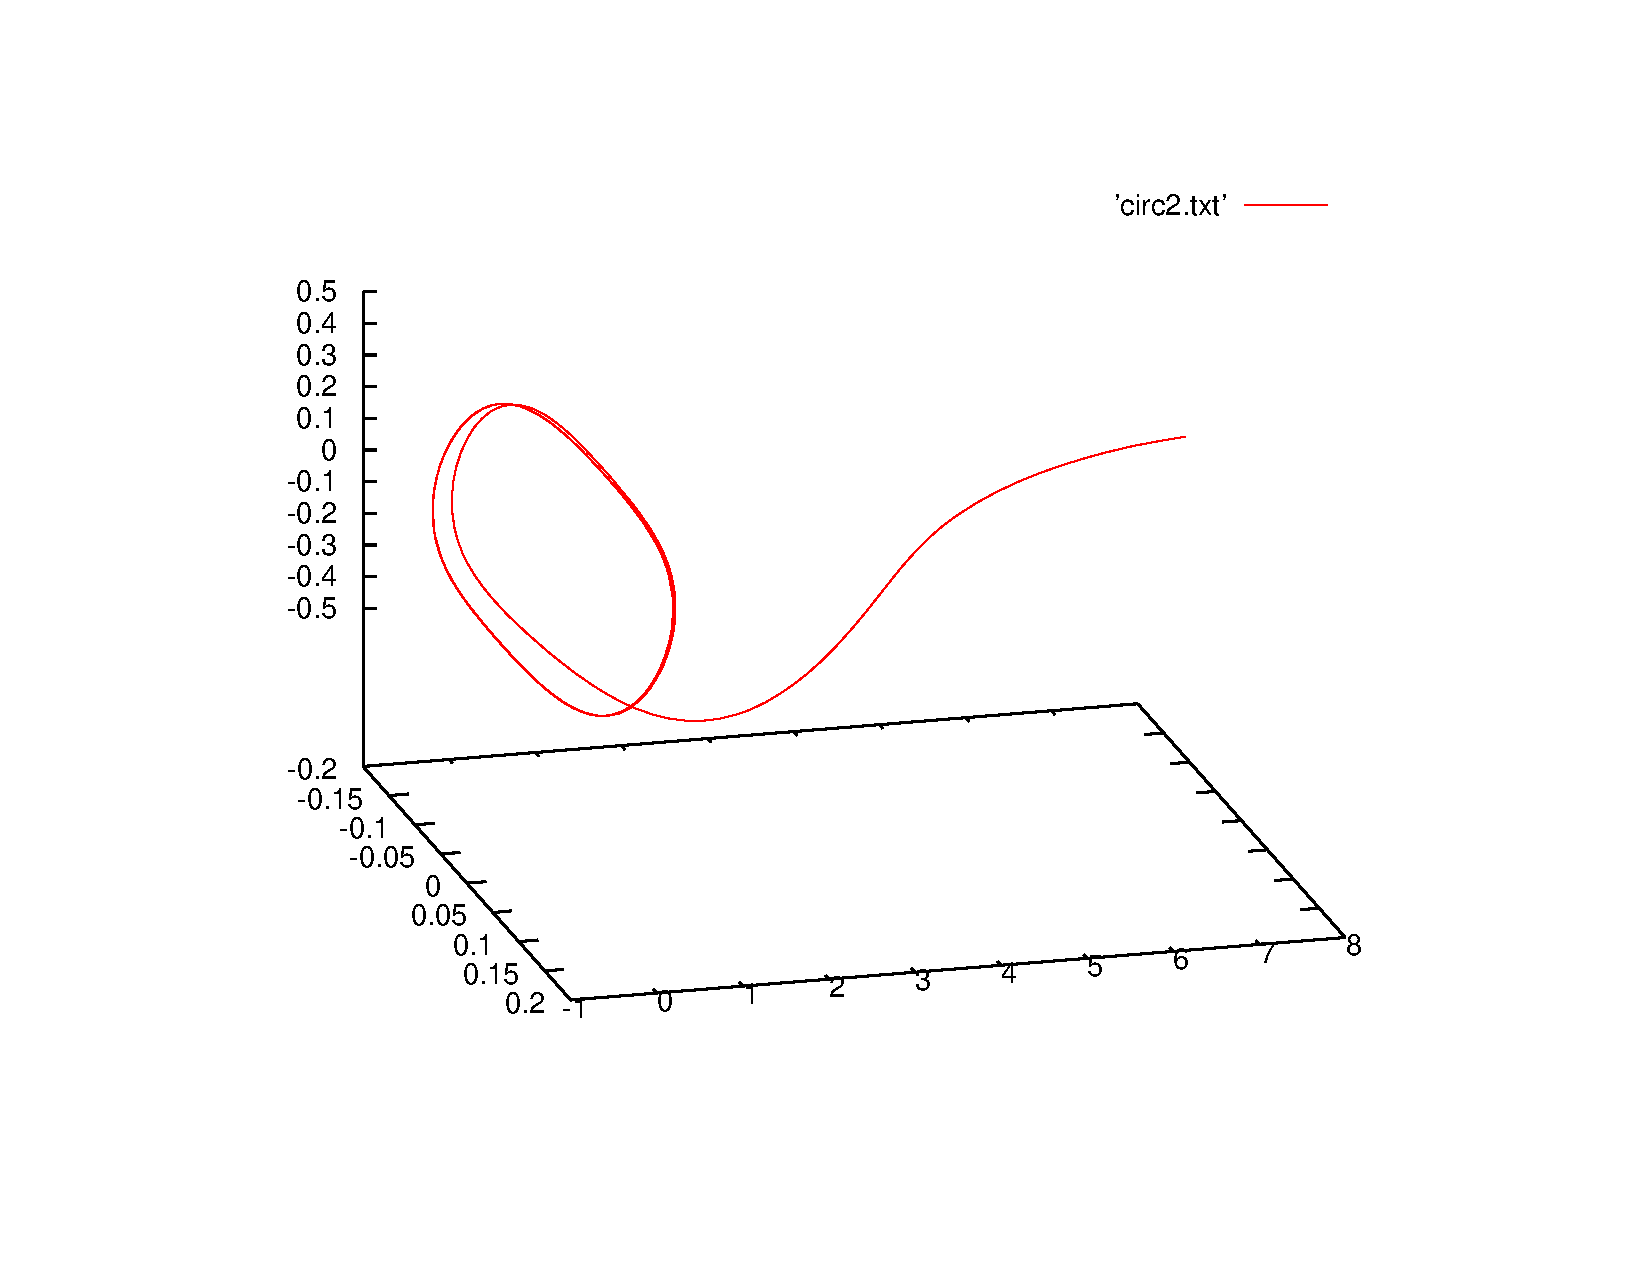
\includegraphics[angle=-90,width=0.6\textwidth]{upo1}
 \caption{the x,y,z axis are the real parts of modes  $a_2$,$a_3$ and $a_4$ respectly. The
 observation time is 170s.}
 \label{xiongupo1}
\end{figure}

Also, when it comes to the wave numbers, I just follow those predecessors.
$k=[0,1,2,...N/2-1,0,-N/2+1,..,-2,-1]$. I don't know why. For me, it
is just a consideration of symmetry. However, Chirs told me it comes from
\textit{Aliasing}. Is he in this blog?

\item[2013-08-23 Xiong Ding]
I tried to used the previous codes\\
\texttt{ksfmetd2.m} and \texttt{ksfmstp.m} in folder \\
\texttt{siminos/matlab/ruslan/}.
However, I got the same result with my code: the trajectory runs away as
in \ref{xiongupo1}.

You can easily check the behaviour of the system:\\
\texttt{\# cd siminos/matlab/ruslan}\\
\texttt{\# octave}\\
\texttt{> [t,y]=ksfmetd2(init,22,0.25,170,1);}\\
\texttt{> plot(t,y(3,:))}\\

where, `init' is a 30*1 vector containing the initial condition for $T_{10.25}$
orbit.

Then you will get a graph like this:
\begin{figure}[h]
 \centering
 \captionsetup{width=.6\textwidth}
 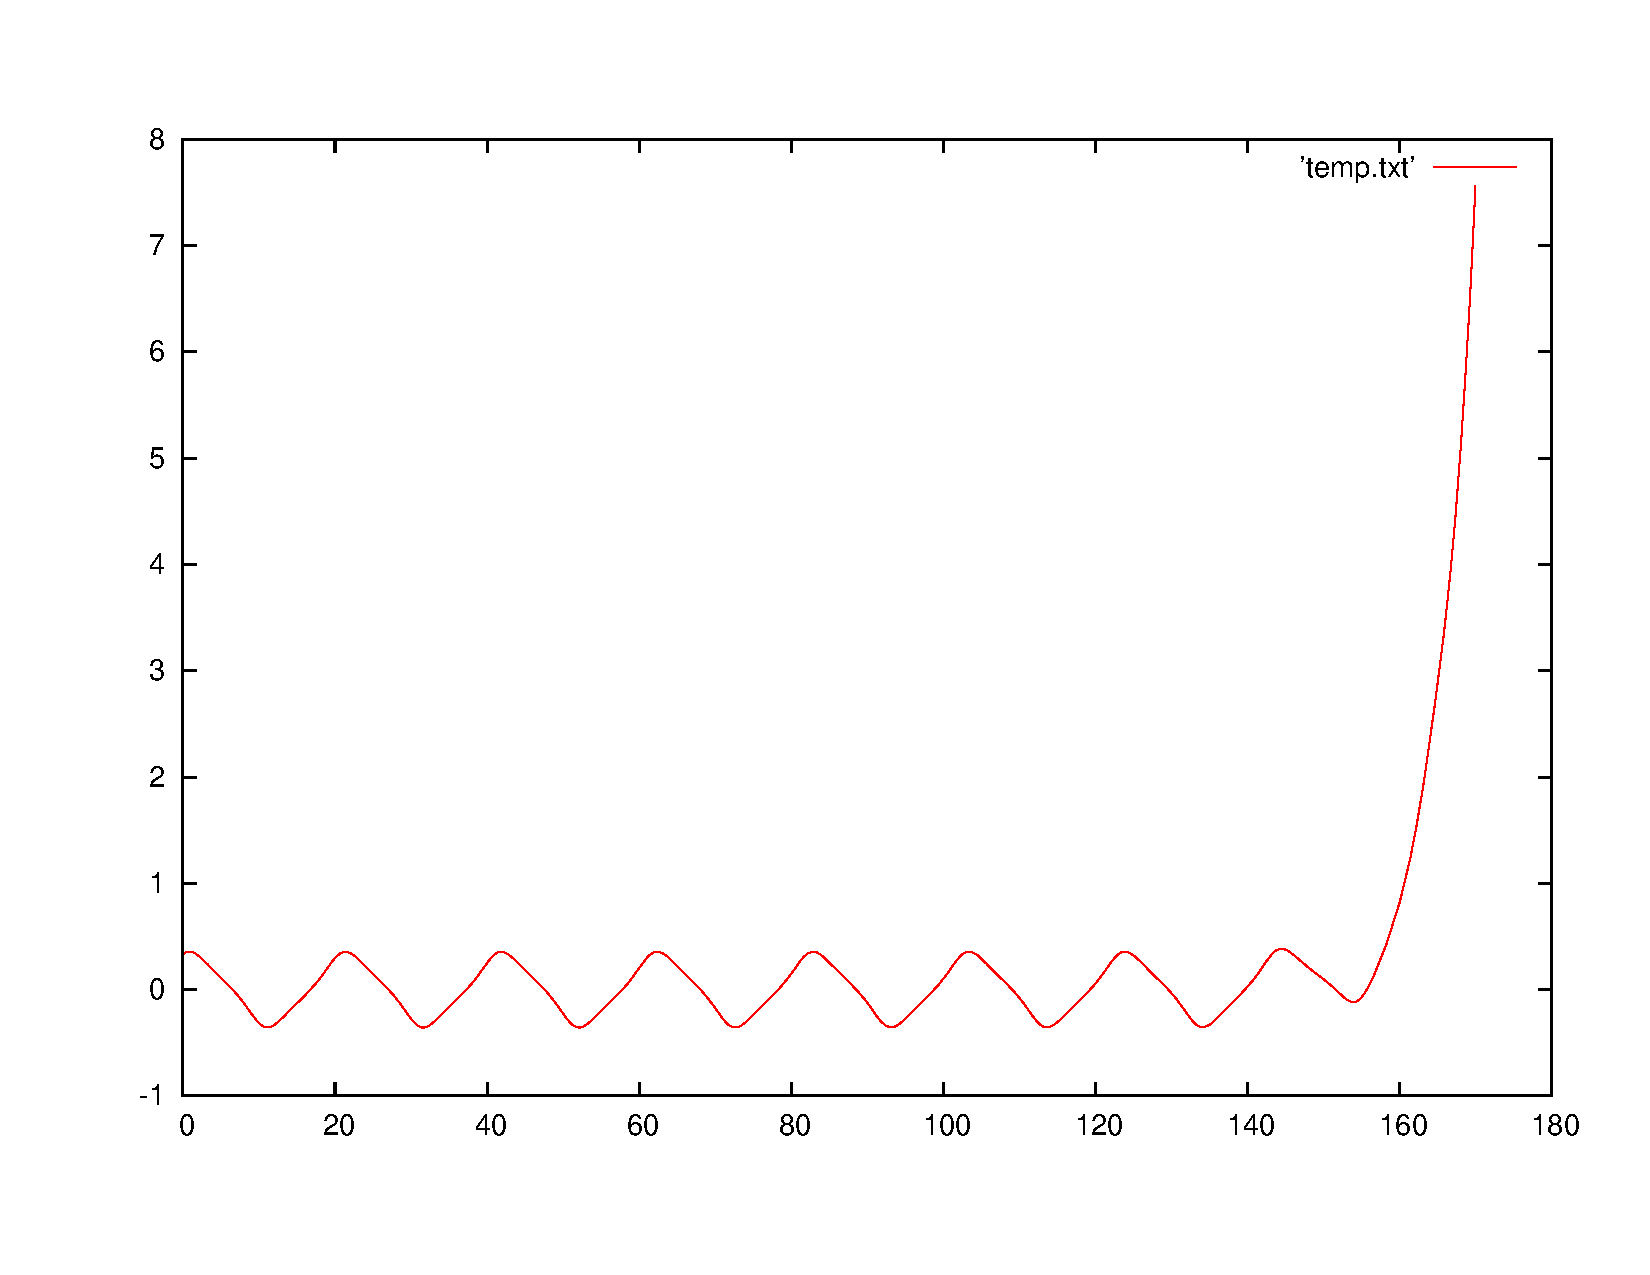
\includegraphics[angle=-90,width=0.6\textwidth]{upo1025_a3real}
 \caption{real part of $a_3$ versus time. the total time is 170s.}
 \label{xiong_upo1025_a3real}
\end{figure}

In about 160s, the real part of $a_3$ begins to run away.
By the way, could my graphs be displayed successfully?

\item[2013-08-02 Predrag to Xiong]
Maybe there is no problem - your trajectory goes somewhere, but
not off to infinity. Start looking whether your spatial plots look right, like
those of \reffig{kaz-evolution}\,(a), and corresponding spatial / time evolution
plots in \refrefs{lanCvit07,SCD07}.

\item[2013-08-23 Xiong Ding]
For the time evolution of the UPO $T_{10.25}$, I got the same figure as in
\reffig{kaz-evolution}. In \refeq{upo1025_statespace}, there are ten
prime periods, so the total time is 102.5s. If the total time is increased,
then this figure collapses. Sorry for bad adjustment of this figure, it takes
a lot of space.

\SFIG{upo1025_statespace}{}{
Xiong's time evolution of \po\ \PO{10.25} for 10 periods,
compare with Kazumasas's \reffig{kaz-evolution}\,(a).}
{upo1025_statespace}

\item[2013-08-23 Predrag]
What do you mean by 'then this figure collapses'?
It is supposed to look like generic turbulence for
$L=22$ system, \reffig{kaz-evolution}\,(c), does it?

\item[2013-08-23 Predrag]
Please, do not put into a repository 1/2\,MB files like
\\
\texttt{upo1025\_statespace.eps},
generate figures of reasonable size (5 to 30\,KB) before committing,
see for example \texttt{siminos/figSrc/00ReadMe.txt}
(add to it, if you learn some good tricks for making figs small).
I replaced it by a 13\,KB \texttt{*.png}. Also, it costs you nothing
to plot them in color, is on page 36 of
\HREF{http://chaosbook.org/overheads/PDEs/UMich07.pdf}
{these overheads}: the result is much prettier.

There is no need to generate \texttt{*.eps} files, small \texttt{*.png}'s are probably all
that is needed for the blog. Otherwise
the repository will become huge in no time. For comparison, entire Oxford publication
version of ChaosBook.pdf
is 4.3\,MB. If I used your figures, it would be 43\,GB :)

I create a new \texttt{00ReadMe.txt} by copying it from some other one,
then editing it, then (in linux, for example):
\begin{verbatim}
svn add 00ReadMe.txt
svn propset svn:keywords "Date Author" 00ReadMe.txt
\end{verbatim}

\item[2013-08-23 Xiong Ding]
Sorry for my carelessness in dealing with figures.

By saying ``then this figure collapses'', I mean the date will increase
monotonously until it reaches the
maximal value of double precision float type (approximate at t=330m),
after which it is stored as: \texttt{NaN (not a number)}.
The figure for $t<300$ is periodic.

\item[2013-08-26 Xiong Ding]
From the description of my project goal, I am supposed to calculate
the stability
( = covariant Lyapunov) exponents associated with \eqva, so I think I
should first try to reproduce Fig~2.2 in \refref{SCD07}, that is why
I am reading \refref{ksgreene88} today. Is it the right way for me?

\item[2013-08-27 Predrag] It is not a pressing issue, but it is
 a good thing to understand the bifurcations of Fig~2.2 in
\refref{SCD07}. You do not want to reproduce the entire graph, but
you certainly should understand bifurcations off the$E=0$ laminar state.
That is analytic, the rest is numerical - do not spend much time on
it.

\item[2013-08-26 Xiong Ding]
Also, last week I tried to calculate the eigenvalues of product of
two matrices: $J=QR$. I don't know how to do it, or should I know? My
method to calculate stability exponents may be awkward.

\item[2013-08-27 Predrag]
The $QR$ decomposition is a standard numerical method described in
many books, referred to in most of the articles you are reading. If
you search for QR in this blog you will find, for example Ginelli
\etal\rf{ginelli-2007-99} as a reference, as well as Dieci
\etal\rf{DJRV07} on QR method (the paper is on
\HREF{http://www.math.ku.edu/~evanvleck/papers.html}
{www.math.ku.edu/$\sim$evanvleck/papers.html}), and many other
references. Does reading of
\refsect{QRdecomp} and \refsect{iscpif} help?


\item[2013-08-27 Predrag]
Have you solved your {\bf [2013-08-23 Xiong Ding]} then ``then this
figure collapses'' problem? I cannot figure out how you could
accurately integrate an unstable \po\ and get decent leading Floquet
multipliers with your code, but have it fail once you leave the that
\po? Mysterious.

Burak can give you a 4\dmn\ system to test your codes on - should be
easier than the full \KS.

\item[2013-08-27 Xiong Ding]
It seems that the problem lies in the \textit{aliasing} of Fast Fourier
Transform. The nonlinear term will produce large wave numbers which
will be aliased to the lower wave number. In this way, the numerical error
will accumulate at lower wave modes. I will try out the ``3/2''
method to solve it. But I am not sure whether it will work or not.

\item[2013-08-28 Predrag] Keeping blogging; for example explain what
is the problem that aliasing fixes? Is this problem not taken care
off in Trefethen, Davidchack, Siminos, and Takeuchi codes? How is it
possible that your code is very accurate on a \po, but fails once you
leave it? That I find very puzzling... There is also a problem of
\KS\ being `stiff'. Have you now read up on the QR decomposition and
understood what is good about it? All this merits writing up. You
have not written up anything that you are learning since {\bf
[2013-08-01 Xiong Ding]}. Two tweets a week are better than none, but
you have to write up important things as you learn them.

\item[2013-08-28 Xiong Ding]
Aliasing is not the problem. I tried to dealias \textit{fft}, but it failed.

I gave up using Octave to run codes now. I tried to use Matlab on
the computer downstairs today, and the data did not run away in Matlab.
Sorry for my embarrassing situation.

\item[2013-08-28 Predrag] Good news. It's life coding - what can you do.
But you lost a month being stuck, so now go back to writing about important
things in life. For example, read, understand (or say what you do not understand)
Daniel's notes and code, compare your Floquet multiplier to his, etc..
Deal with open questions above that you never closed. Let's
get back on the roll, start looking at different \po s / \rpo s and
connecting them with their stable / unstable manifolds. Etc.

\item[2013-08-30 Kazumasa]
Great! (though it must sound frithening to those using Octave... not me!)
Xiong, have you also computed Floquet multipliers?
(Predrag's treets suggest you did, but I can't find...)
I'm wondering how many multipliers you can compute accurately
 with the method you use.
Strongly contracting directions result in nearly zero eigenvalues (multipliers)
 of the Jacobian, which are then much more difficult
 to estimate numerically than those for expanding directions.
For comparison, you can find a list of ``Lyapunov exponents''
 [$=(1/\text{period})\log\text{(Floquet multiplier)}$] of this orbit at\\
\texttt{siminos/kazz/data/UPOa-lyap.dat} .

This problem will be more severe when you want to measure longer orbits
 (remember that \PO{10.25} is the shortest we have),
 but it is those multipliers / eigenvectors that may play an important role
 when we try to construct the dimension of the inertial manifold from orbits
 (if you don't see what I mean, have a look at \refrefs{YaTaGiChRa08,TaGiCh11}
 -- constructing the inertial manifold in terms of orbits
 is one of the (ultimate) goals of the project, at least to Hugues and me).

 \item[2013-08-30 Xiong Ding to Kazumasa]
 Thank you for your suggestion. I will read \refrefs{YaTaGiChRa08,TaGiCh11}.
 My Floquet multipliers are posted in \reftab{xiong_fe1025}. My result is
 very crude, and the exponents corresponding to strongly contracting directions
 are totally wrong. I just evolve the system for one period (20.50s), and then
 calculate the eigenvalues of the Jacobian matrix. Therefore, I get 32 exponents.
 Since the eigenvalues expand a huge range and I don't know how to control
 precision, my result is by no way reliable. Your smallest exponent is
 about $-90$, so the corresponding eigenvalue is about $exp(-90*20.50)$.
 What did you do to get the exponents precisely?

 I read your file \\
 \texttt{siminos/kazz/data/UPOa-lyap.dat}\\
 Why do you have 23 exponents?

\item[2013-08-30 Kazumasa to Xiong]
Thank you for referring me to your data set.
This is what I anticipated and an annoying problem
 when computing Floquet exponents from the Jacobian matrix...
In my case, I used the Gram-Schmidt algorithm
 (or equivalently the QR decomposition) to compute the exponents,
 as if to compute Lyapunov exponents of a chaotic trajectory
 (with a small trick to keep the trajectory ``trapped'' on the orbit).
This is a great advantage of the Gram-Schmidt method,
 because one can shorten the time step as much as one wishes
 so as to achieve a desired precision of the computed exponents.
The time step I chose for computing the posted exponents was 0.005,
 for which the vector associated with the exponent $-90$ shrinks
 on average by the factor $\exp(-90 \times 0.005) \approx 0.64$,
 and I performed the Gram-Schmidt orthogonalization
 at every 40 time steps, for which the shrinking factor is
 $\exp(-90 \times 0.005 \times 40) \approx 10^{-8}$,
 still sufficiently above the machine precision.

One can compute as many exponents as one wishes by increasing the number
 of Fourier modes and collocation points.
For the Gram-Schmidt method, the number of the exponents is also limited
 by the time step you choose (this is the advantage I've just mentioned).
In my case I chose the time step that gave me the first 23 exponents reliably,
 and I didn't want to shorten the time step further
 to compute more unnecessary exponents by spending longer time
 (the chaotic trajectories of the KS equation for $L=22$ has
 9 physical exponents,
 ``physical'' in the sense of \refrefs{YaTaGiChRa08,TaGiCh11},
 while the remaining exponents are all conjectured to be
 unnecessary to describe the dynamics... but we need to compute
 at least some of these unnecessary modes for our project).

Anyway, I think you/we should consider
 how to compute negative exponents reliably
 (not necessarily up to -90, but hopefully to -10),
 if you prefer using the Jacobian.
I guess you can implement the Gram-Schmidt method
 on the Trefethen algorithm when needed.

 \item[2013-09-02 Xiong Ding to Kazumasa]
 Thank you for all the valuable information. Now I realize the value of
 analyzing what precision I could get before running the code.

 I have tried to
 use QR decomposition before, and
 the formula of the exponents I used is:

 \[
 \lambda_i=\lim_{T\to \infty} \frac{1}{T} \sum_{h=0}^{T-1}
  \ln\gamma_{k,n+hk}^{(i)}
 \,.
\]

However, I gave up after several trials because the trajectory began to
depart from the \po\ around 400s.
The problem may lie in my implementation of
Trefethen's algorithm, but it still exits when the time
step was reduced to 0.005s. So I am curious what kind of trick you used to keep the trajectory
trapped on the orbit?

\item[2013-09-02 Ruslan to Xiong Ding] The orbit is unstable, so you cannot expect
for the numerical solution (whatever the numerical method) to stay on it forever.
The trick is to integrate it only for as long as necessary, i.e. up to its period,
and then re-use these points as necessary.
Kazumasa wrote about this somewhere else in
this blog and this is what Daniel does as well.

\item[2013-09-02 Xiong Ding to Ruslan]
The trick requires me to know the exact period.

\item[2013-09-02 Predrag to Xiong Ding] It's not a trick, a \po\ is a compact set
of periodic points, so staying on it is perfectly legal - and for very unstable orbits
mindless integration forward in time might be impossible even for a
single period (see complex Lorentz flow in ChaosBook, Siminos thesis, etc:
the full \statesp\ \reqv\ cannot be integrated for 1 period).
You just check every so often how far are
you from the (numerically) exact \po, and reset your point
$\ssp(\zeit)$ to it, if you have started to stray off.
You have 18 significant digits of $\period{p}$,
Floquet multiplier along of the flow is exactly 1, so it would take
a very long time to lose accuracy in time. As to exact period,
(re)read my {\bf [2013-07-30 Predrag to Xiong]} comment.
You write above:
``I just evolve the system for one period (20.50s)''. This is a
`preperiodic', or \rpo\ whose period is $\period{}=10.25336729174627$
in the time units defined by the form of \KSe\ you chose to use
(see \refeq{eq:GKscale}, for example). Seconds are used in
cardiac dynamics, if your parameters are physiological ones, but
usually one non-dimensionalizes one's equations as the first
step, to count the parameters. You traverse the orbit twice. Here
the orbit is short, so does not matter much, but later on already
twice the period might suffice to lose the orbit.

\item[2013-08-29 Xiong Ding to Evangelos] I have a simple question about Lyapunov exponents.
You set the truncation number $N=64$, and you get 62 Lypunov exponents.
I am confused why the number is two less than the dimension. Are the extra zero?

\item[2013-08-30 Evangelos to Xiong Ding] Do you refer to Ruslan's matlab code
in your question? The answer is probably related to the fact that there are
two Fourier modes (zero and the last one) that are set identically equal to zero.

\item[2013-08-31 Xiong Ding to Evangelos] Yes, I am referring to Ruslan's code.
He sets the wave number to be $[0:N/2-1, 0, -N/2+1,-1]$,
so the time derivative of  tangent vector $b_0$ and $b_{N/2}$ is zero.
These two vectors will not expand or contract.
Therefore, the corresponding exponents are zero,
but my problem is that $b_0$ and $b_{N/2}$ will be changed after
QR decomposition. I don't know whether this is a problem.

\item[2013-09-02 Evangelos to Xiong Ding] I think that you should not include
$b_0$ and $b_{N/2}$ in your calculation of the Jacobian (i.e. you should work
with a $(N-2)\times (N-2)$ matrix right from the outset. Maybe someone could
verify or dispute this point?


\item[2013-09-02 Ruslan to Xiong Ding]
I think it would be good for you, Daniel,
me and Predrag to have a discussion (over Skype or Zoom), so we can come to a common
understanding of what we are trying to do and what's the best way forward.

\item[2013-09-02 Xiong Ding to Ruslan] Thanks.
I will contact Prof. Predrag to arrange a webinar
between us, and hope it will be held in this week as soon as possible.
My progress is very slow!

\item[2013-09-02 Predrag] Good idea. Xiong Ding, go ahead and propose a
when to meet, try to find time good for all. Blog it, so
other collaborators can join if they want to. Skype is fine if we only talk; if we
want to show slides, formulas, etc, WebEx is better - Xiong Ding can learn from
Chris how to schedule a meeting. My calendar is on my home page; Wednesday
cardiac group meets at 11am, so we have to finish by then.

We are planning to have Daniel do a webinar presentation of his work
(Tue 10am New York time,
3pm in England, 4pm in Germany), but the study group is not ready for that yet.

\item[2013-09-02 Predrag to Xiong Ding]
Please study and write up here, or in \refsect{sect:introXD} \ABedit{by Thursday night}
(see {\bf [2013-08-18 Predrag]} above, etc.) your understanding of
(\HREF{../crane/CalculatingCLVs.pdf} {click here}) first installment of Daniel's saga.
Working assumption for Ruslan and me is that what ever you have not written
down, you have not studied and/or understand, and if you are not prepared,
we are not going to get much out of a meeting.

\item[2013-08-31 Xiong Ding to Daniel Borrero]
My code is not written in a flexible form, so I need to define the function for the \KS\ system. One of my major problems is the control of precision. I got a similar result as Siminos, but I don't think my result is reliable because the exponents are reluctant to converge in my code. Last time, I saw your post in the blog, saying that the Lyapunov eXPONENTS you got are well fitted to $(q^2-q^4)$, so I assumed that you are working on \KS\ system, but I was wrong.

I will try to read your code and apply it to \KS\ system.

\item[2013-09-03 Daniel B to Xiong Ding]
I don't know if I would necessarily waste my time calculating Lyapunov exponents in the sense that is calculated in my code. That was state of the art in 1985 but there are much smarter things to do in 2013. The reasons why Lyapunov exponents in the sense calculated in my code are the wrong thing to calculate is explained  \HREF{http://www.streamsound.dk/book1/chaos/chaos.html\#137/z} {here}. As far as I know there is no direct way to compare this kind of Lyapunov exponents with the results that you would get from covariant Lyapunov vectors, so I think the very best, you might find that you have the same number of unstable and stable ones, but they won't be related in any way. I just did what I did because it was an easy, dirty way to figure out whether my parameter set was giving me chaotic dynamics but like I wrote in the blog, it probably doesn't do much more than that. I think Predrag would be WAY happier if we computed covariant Lyapunov vectors for our 4D system, than Lyapunov exponents for your 64D system, so I would put my efforts there.

Then again, it quick and easy, feel free to try and implement it. It shouldn't be too hard to generate the extended ODE system automatically. It might take a while to compute for a 64 dimensional system...


\item[2013-09-03 Predrag to Xiong Ding]
I realize thinking is extra cost, but there is no substitute for it - coding comes only \emph{after} one has understood the theory, it is an implementation of one's understanding.
We were computing \jacobianMs\ like you do in 1996\rf{Christiansen97}. Since
2007\rf{ginelli-2007-99} the community has a better method\rf{GiChLiPo12}. It's unlikely
you would reinvent it on your own, as it took more than 20 years to get to the
present state, and that is not for the lack of codes, but for the lack of critical
rethinking.

As long as you avoid to do what a scientist must do - sit down in a quiet room with the printed paper of \refref{GiChLiPo12}, a pencil and a pad, work through every line of the paper and understand it, and reemerge after you have mastered it, you cannot code anything, and getting someone's else code will only hamper your progress in the long run.
There is no short cut to understanding - every great physicist that we know of
works very hard to come up with something simple and beautiful, from the guy with
wild white hair to Feynman to Shina Tan.

Once you have mastered the current state of art, you can lean back and start dreaming. I have a concrete suggestion {\bf [2013-08-19 Predrag to Daniel]}, but maybe you will do something truly elegant instead. But if you cannot play the instrument, you cannot make beautiful music.


\item[2013-09-29 Daniel to Xiong]
I apologize for not having written in the blog for a while, I've had a busy few weeks - and unfortunately right now I'm in the middle of writing an end of year report to summarise my progress. Once I'm done with this report, I'll hopefully work on finishing up the documentation of my code, which will mostly be concentrating on how I used the CLV method of Ginelli et al. to calculate the stretching rates (which correspond to the Floquet Eigenvalues) of the CLVs. I'll also try to post up some examples of the results that I get for some of the shorter RPOs/PPOs, so that you can compare results.

I noticed that you were confused about why I needed to calculate the matrix \textbf{D} in my script - which was in fact a great point, as it's completely unnecessary for us to use this diagonal matrix \textbf{D} since we're normalising the columns of \textbf{C} at each step anyway. I've updated my code to remove \textbf{D} accordingly, and will update the documentation to match. Thanks for pointing this out!

I was wondering if you have any other questions that you'd like for me to answer regarding my workings?

\item[2013-10-05 Xiong to Daniel]
Sorry to reply you so late. I uploaded my Matlab code in \texttt{siminos/xiong/matlab} and the local Lyapunov exponents for the orbit $T_{10.25}$.
It seems that your code calculates the Floquet exponents, but I calculated the Lyapunov exponents. What confused me is the number of exponents.
If I set truncation number $N=32$, then I will get $32$ exponents because the flow in tangent space is 32-dimensional, but you get $30$. I know one exponent should be zero due to symmetry (which I haven't implemented yet), but what about the other one? Can you recommend some paper for
me to read?

\item[2013-10-07 Daniel to Xiong]
I believe that this is explained in Appendix A of \refref{SCD07}. It's because the first Fourier mode is set to 0, and stays there - meaning that $a_0 = b_0 + ic_0 = 0$.

\item[2013-10-11 Xiong to Daniel]
$a_{0}$ is just a real number.  Should ther reason be that both $a_{0}$ and$a_{N/2}$ are zero ?

\item[20313-10-22 Xiong to Daniel]
I have a problem recently with Ginelli \etal\ method.  In the forward transient stage, we evolve the state in the tagent space and
conduct $QR$ decomposition very certain time interval. The purpose of this stage is to make the orthonormal basis $g_{n}^{(i)}$
converge to eigenvectors ${(d_{n}^{(i)})_{-}}_{i=1,\cdots,N}$ of the backward Oseledets' matrix. But what I found is that
$g_{n}^{(1)}$, $g_{n}^{(2)}$, $g_{n}^{(6)}$ and $g_{n}^{(7)}$ do not converge. $g_{n}^{(1)}$ and $g_{n}^{(2)}$ are rotating
in a two-dimensional subspace and the rotated angle is different from cycle to cycle. The same is with $g_{n}^{(6)}$ and
$g_{n}^{(7)}$.

I guess the reason is that the first and second eigenvalues are degenerate, the same goes with the sixth and seventh
eigenvalues. Do you have same problem? How do you handle it?

\item[2013-10-24 Predrag] Complex eigenvalue / eigenvector pairs
is the second thing (after discussing the non-degenerate
case) that methods for
finding eigenvectors by multiplication along the trajectory
must deal with. Does this paper by
\HREF{http://journal.taiwanmathsoc.org.tw/index.php/TJM/article/view/336}
{Ruhe}\rf{Ruhe10} answer your question?

There is this secret fraternity of
nerds called `Google' that has lots of suggestions: search for `complex' in
\HREF{http://books.google.com/books?hl=en&lr=&id=wE0NrHkrqRAC&oi=fnd&pg=PR11&dq=Krylov+method+\%22complex+eigenvalues\%22&ots=t1Gb0AGWN4&sig=KVftvLx0yoczpXG7EMfAgFOWxr4\#v=onepage&q=complex\%20eigenvalues&f=false}
{here}, or
\HREF{http://www.siam.org/books/ot101/OT101Sample.pdf} {here}, or ....
If Lyapunov is your thing,
\HREF{http://www.science.gov/topicpages/l.html\#target765} {try this:)}

\item[2013-10-29 Predrag] Reading {Ruhe}\rf{Ruhe10} we learn that
the complex eigenvalue pair case is treated by `the double shift
QR or QZ algorithm'. It is probably in {\em  Numerical Recipes}\rf{nr},
in Golub and Van Loan\rf{GoVanLo96}, or any other text on QR decomposition such as \HREF{http://people.inf.ethz.ch/arbenz/ewp/Lnotes/chapter3.pdf}
{this one}, randomly spewed out by Google.

\item[2013-11-10 Xiong Ding]
Sorry for not updating the blog for long time. The Lyapunov exponents I got are documented in the figure below. For the first, second, sixth and seventh
exponents, the averaged value converges very slowly, So I use large time step $h=T/50$,
where $T$ is the prime period $10.25\cdots $, to get the first 10 Lyapunov exponents, but for the remaining
ones, I used small time step $h=T/2000$.

\begin{figure}[h]
 \centering
 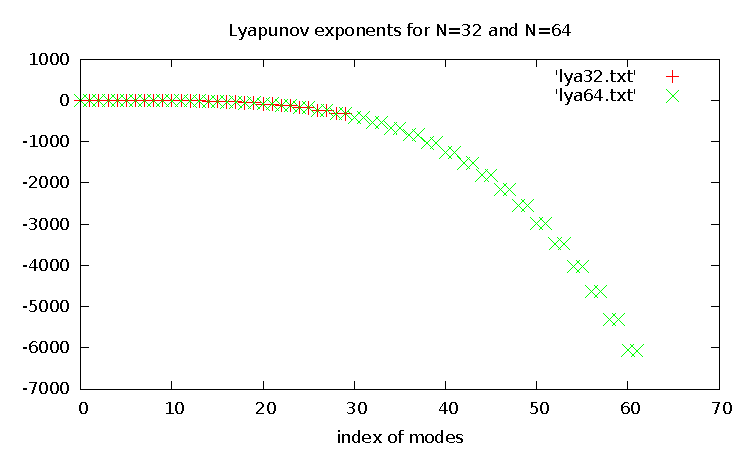
\includegraphics[width=0.8\textwidth]{lyaExp.pdf}
 \caption{Lyapunov exponents for for trunction number N=32 (red) and N=64 (green).}
 \label{fig:lyaExp}
\end{figure}

When evolving the system in tangent space, I conduct QR decomposition regularly. The Gram-Schmidt vectors should
converge to the backward Oseledec vectors ( eigenvectors of backward Oseledec matrix). However, what I found is not
converging vectors but converging subspaces, which are due to the complex pair of eigenvalues of Jacobian matrix. Each such
subspace consists of two rotating vectors.  From my code, only the 5th and 8th vectors are not rotating.  I computed the convergence
of subspace in Fig \ref{fig:diff_subspace}. The residue of projecting one subspace onto another one is very small, so these
sbuspaces converge.

\begin{figure}[h]
 \centering
 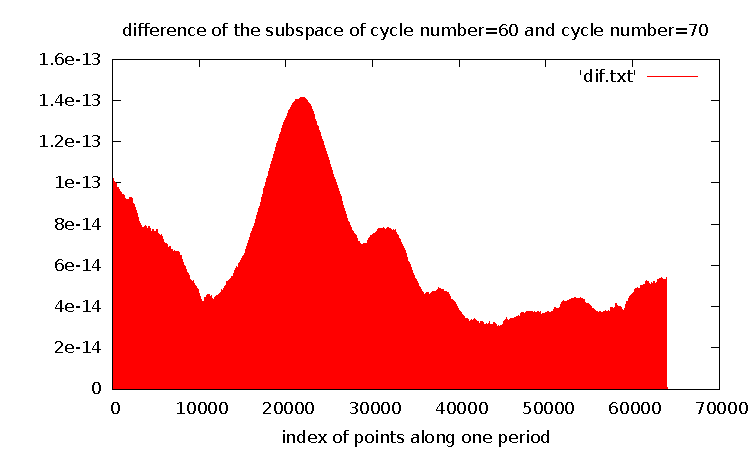
\includegraphics[width=0.8\textwidth]{diff_subspace.pdf}
 \caption{I computed the Gram-Schmidt vectors of cycle 60 and those of cycle 70. The convergence is computed as following:
 let the index of vectors be $i$, which can be $1,2,3, \cdots , 30$. If $i\neq 5  $ and $i\neq 8$,  then $v_{i}^{(70)}$ and
 $v_{i+1}^{(70)}$  is projected to  the subspace spanned by $v_{i}^{(60)}$ and  $v_{i+1}^{(60)}$,  $ i=1,3,6,9,11,\cdots ,29$
 and then the norm of the residue is
 recorded. If $i=5$ or $i=8$, then the subspace is one-dimensional, then $v_{5}^{(70)} $ is projected onto $v_{5}^{(60)} $
  and $v_{5}^{(70)} $ is projected onto $v_{5}^{(60)} $.}
 \label{fig:diff_subspace}
\end{figure}

I got the Covariant Lyapunov vectors and tried to verify whether they are correct or not.  I think Covariant Lyapunov
 vectors should satisfy two conditions: First the expansion or
contraction rate of these vectors should be the corresponding Lyapunov exponents.  The asymptotic forward Gram-Schmidt vectors
also satisfy this requirement, so we need at another criteria.
Second, the Covariant Lyapunov vectors should vary consistanly as system evoles, that
is
\begin{equation}
v(x_2, t_2)=J(t_2, t_1)v(x_1, t_1)
\label{eq:clv_consistance}
\end{equation}

without Gram Schmidt orthogonization.  $v(x_2, t_2)$ and  $v(x_1, t_1)$ are Covariant vector
 at position $x_2$ ,  $x_1$ and time $t_2$, $t_2$ respectively. Since the first asymptotic forward Gram-Schmidt vector
is just the first Covariant Lyapunov vector, it satisfies this requirement, but others do not.  I checked whether my Covariant Lyapunov
vectors satisfy  \ref{eq:clv_consistance}, and my result shows that the maximal norm of
$v(x_2, t_2)-J(t_2, t_1)v(x_1, t_1)$ is around $10^{-5}$.
I don't know whether it is good enough.

\item[2013-11-18 Xiong Ding]
I used the \textit{Periodic Schur decompostion}\rf{Bojanczyk92theperiodic}
to calculate the Floquet exponents and covariant vectors. This method has been
documented before,
% on page \pageref{ruslanperiodic}
see \refchap{sect:LyapKS}, entry  {\bf 2009-09-12 Ruslan}.  Did Ruslan implement this method
before?

\item[2013-11-20 Ruslan] Yes I tried it. I used routine MB03WD in the \HREF{http://slicot.org/objects/software/shared/libindex.html}{slicot.org} library.  But for some reason it did not work.  Some of the RPO and PPO eigenvalues appeared correct, while others did not.  I don't remember the details now.

\item[2013-11-20 Predrag] Day before yesterday Xiong Ding showed up
clutching a secret, un-blogged piece of paper, which seemed to contain
a table of all Floquet exponents and eigenvectors for the second repeat of
the relative prime orbit \PO{10.25} to machine precision.

For \KS\ this seems to obviate the need for computing these things by
`covariant vectors' methodology of
\refref{GiChLiPo12}; have precise Floquet vectors and can implement the grand
plan of the Skype Supreme Plenum of {\bf 2013-10-18}.
However, no one seems to evince a slightest interest into the {\e To do list} of
\refsect{sect:ToDo}, and Xiong Ding will spnd next two weeks doing his
project for the parallel computation course.





\end{description}

\renewcommand{\ssp}{a}
